\documentclass[11pt,a4paper]{article}
\usepackage[T1]{fontenc}
\usepackage[utf8]{inputenc}
\usepackage{lmodern}
\usepackage[margin=26mm,headheight=15pt]{geometry}
\usepackage{amsmath,amssymb,amsthm,mathtools}
\usepackage{booktabs,longtable,array}
\usepackage{xcolor,microtype,enumitem,fancyhdr,hyperref,pdfpages}
\hypersetup{colorlinks=true,linkcolor=blue!40!black,urlcolor=blue!45!black,
 citecolor=blue!40!black,pdftitle={Constructive Isoperimetry in Intuitionistic Primitive Recursive Arithmetic},
 pdfauthor={Research report prepared for Vladimir Reshetnikov}}
\pagestyle{fancy}
\fancyhf{}
\fancyhead[L]{\small Constructive isoperimetry in iPRA}
\fancyhead[R]{\small Finite proofs and effective geometry}
\fancyfoot[C]{\thepage}
\setlength{\parskip}{4pt}
\setlength{\parindent}{0pt}
\setlist{itemsep=3pt,topsep=5pt}
\setlength{\emergencystretch}{2em}
\allowdisplaybreaks
\newtheorem{theorem}{Theorem}[section]
\newtheorem{lemma}[theorem]{Lemma}
\newtheorem{proposition}[theorem]{Proposition}
\newtheorem{corollary}[theorem]{Corollary}
\theoremstyle{definition}
\newtheorem{definition}[theorem]{Definition}
\newtheorem{remark}[theorem]{Remark}
\newcommand{\ipra}{\mathsf{iPRA}}
\newcommand{\N}{\mathbb N}
\newcommand{\Q}{\mathbb Q}
\newcommand{\R}{\mathbb R}
\newcommand{\eps}{\varepsilon}
\newcommand{\abs}[1]{\left|#1\right|}
\newcommand{\norm}[1]{\left\|#1\right\|}

\begin{document}
\hypersetup{pageanchor=false}
\begin{titlepage}
\vspace*{12mm}
{\color{blue!45!black}\large MATHEMATICAL RESEARCH REPORT\par}
\vspace{7mm}
{\LARGE\bfseries Constructive isoperimetry\\[3mm]
in intuitionistic primitive\\[3mm] recursive arithmetic\par}
\vspace{9mm}
{\large Planar and higher-dimensional inequalities,\\
Wigner caustics, triangles, and hypercube boundaries\par}
\vspace{10mm}
Prepared for Vladimir Reshetnikov\\
15 November 2026
\vspace{8mm}
\begin{abstract}
We develop constructive versions of the mathematical statements in the
Wikipedia article \emph{Isoperimetric inequality}. The finite core consists
of explicit rational or integer inequalities: polygonal isoperimetry,
both triangle inequalities, a rational-parameter Brunn--Minkowski theorem
for finite unions of boxes, Fourier deficit identities, the sharp hypercube
edge inequality, and the full Harper vertex theorem. The proof of the box
theorem uses exact rational volume cuts with a bounded recursion; the
hypercube proof includes the exceptional compressed families.

The finite results extend to specified primitive recursive geometric
presentations, with all approximation and regularity hypotheses stated.
These yield the sharp planar inequality and circle rigidity, the
Wigner-caustic improvement and constant-width equality, sharp Euclidean
isoperimetry with an outer-volume modulus, a finite layered Sobolev theorem,
and spherical inequalities for finite unions of caps and their complements.
We distinguish these results from unrestricted classical claims that this
report does not prove. The Lean contribution specifies finite definitions,
internal iPRA proof targets, and a concrete completion path; it is an
uncompiled outline rather than a finished formal proof.
\end{abstract}
\vfill
\begin{tabular}{@{}p{0.24\textwidth}p{0.68\textwidth}@{}}
\toprule
Human proof & Full finite arguments and explicit presentation-dependent
transfer estimates.\\
Foundation & Intuitionistic first-order PRA with quantifier-free induction;
ProveIt APIs audited at an immutable commit.\\
Artifact status & LaTeX and compiled PDF, original planar appendix,
Lean outlines, exact-arithmetic reference code and validation records.\\
Formal status & No completed internal Lean derivation is claimed.\\
\bottomrule
\end{tabular}
\end{titlepage}
\hypersetup{pageanchor=true}
\pagenumbering{roman}

\setcounter{tocdepth}{1}
\tableofcontents
\clearpage
\pagenumbering{arabic}

\section{Results, coverage, and the meaning of the claim}

The request concerns a broad article, ranging from elementary triangles
to geometric measure theory. The appropriate constructive answer cannot
be a single invocation of its classical results. We give exact finite
theorems first, then state the data needed to interpret them geometrically.
The article was consulted on 15 November 2026 \cite{Wikipedia}; the
mathematical proofs below are developed in full, with primary references
for the classical results and exact provenance for the reused repository
work.

\begin{longtable}{@{}p{0.29\textwidth}p{0.61\textwidth}@{}}
\toprule
Article topic & Result proved here and its scope\\
\midrule
\endfirsthead
\toprule Article topic & Result proved here and its scope\\\midrule
\endhead
Planar inequality & \(4\pi|A|\leq L^2\) for explicitly represented
boundaries; a uniform rational-polygon theorem; circle rigidity for the
effective parametrized class. The full prior finite proof is appended.\\[3pt]
Quotient, ratio, optimizers & \(Q\leq1\), \(L^2/A\geq4\pi\),
disk attainment, equivalence of the fixed-length and fixed-area problems,
and Dido's semicircle optimum, with positive denominators specified.\\[3pt]
Regular polygons & The exact formula \(Q_n=\pi/(n\tan(\pi/n))\),
strict increase, and \(0<1-Q_n\leq8/n^2\).\\[3pt]
Wigner-caustic refinement & Full finite support-polynomial proof and
effective \(C^2\) support-function extension; equality exactly at constant
width within that class; an explicit width-stability estimate.\\[3pt]
Euclidean dimensions & Root-free Brunn--Minkowski for rational box unions;
\(P^n\geq n^n\omega_nV^{n-1}\) for explicit outer-volume presentations;
verified box-union and ball examples; balls attain equality.\\[3pt]
Sobolev connection & Finite layered and cubical BV inequalities with the
sharp constant; an explicit sufficient approximation contract for the
analytic \(W^{1,1}\) form. Universal effective coarea is not asserted.\\[3pt]
Sphere & Exact cap equality; the spherical inequality for finite disjoint
cap unions and their complements; radius scaling and complement symmetry.
The general spherical curve theorem is not proved.\\[3pt]
Finite graph profiles & Bounded algorithms computing edge and vertex
profiles and returning minimizing subsets.\\[3pt]
Hypercube edge boundary & Full sharp edge inequality in an integer-power
form, subcube equality classification, and sharp half-volume expansion.\\[3pt]
Hypercube vertex boundary & Full Harper theorem for every size, binomial
thresholds, exact boundary at Hamming-ball sizes, and all-distance
neighborhoods.\\[3pt]
Triangles & Both inequalities in the article, equivalent radical-free
polynomial inequalities, and equilateral equality for nondegenerate
triangles.\\[3pt]
Other generalizations & No unrestricted theorem about arbitrary Hadamard
manifolds, arbitrary metric-measure spaces, general Hausdorff/Minkowski
boundary identifications, or all higher-dimensional equality sets is
claimed.\\
\bottomrule
\end{longtable}

\paragraph{Organization and reuse.}
The arithmetic conventions come first. The planar section summarizes and
audits the decisive finite argument already in ProveIt, then adds the
regular-polygon and Wigner developments. The box, Sobolev, spherical,
hypercube, and triangle sections give their own complete proofs. The
repository section states exactly which Lean definitions exist and which
proof terms remain to be built. Appendix~\ref{app:planar-full} reproduces
the complete 22-page upstream planar paper, with its original provenance
and original uncompiled-Lean status preserved. This report is therefore
readable without downloading an additional paper from the repository.

\section{What an isoperimetric theorem means in intuitionistic PRA}
\label{sec:foundations}

The first-order language of \(\ipra\) has natural-number variables, symbols
for primitive recursive functions, and intuitionistic logical operations.
It does not have a sort containing all subsets of \(\mathbb R^n\), all
continuous functions, or all real numbers. Accordingly, there are two
precise kinds of result in this report.

\begin{enumerate}
\item A \emph{uniform finite theorem} has arbitrary natural-number inputs
encoding rational numbers, finite lists, graphs, or boxes. Its hypotheses
and conclusion are decidable comparisons, or explicitly displayed
first-order formulas built from them.
\item An \emph{effective geometric theorem schema} fixes primitive
recursive names and moduli, possibly with additional numerical parameters.
The theorem then concerns all those parameters and all requested
precisions. A name is never evaluated by a supposed universal total
evaluator for arbitrary primitive recursive programs.
\end{enumerate}

This distinction is essential. There is no primitive recursive universal
evaluator for all primitive recursive programs: a diagonal program would
contradict its universality. Fixing a family of programs, or accepting
bounded computation traces, is legitimate; silently quantifying over
arbitrary functions and evaluating them is not.

\subsection{Coding and order}

Encode an integer by its sign and magnitude and a rational by an integer
numerator and a positive denominator. Comparisons use cross products;
normalization by the Euclidean algorithm is optional. Finite lists have
a length and bounded access functions. Products, sums, bit operations,
bounded minimization, and finite sorting are primitive recursive.
The displayed rational inequalities can therefore be cleared of positive
denominators and read as integer inequalities.

A named real \(x\) is a fixed primitive recursive rational sequence
\(x[k]\) with a proved Cauchy estimate, for example
\[
 |x[j]-x[k]|\leq 2^{-j}+2^{-k}\quad(j,k\in\mathbb N).
\]
The intended value satisfies \(|x-x[k]|\leq2^{-k}\). This latter notation
is explanatory shorthand: every argument can instead use the preceding
rational comparisons. Define
\[
 x\leq y\quad:\Longleftrightarrow\quad
 (\forall k)\ x[k]\leq y[k]+2^{1-k},
\]
after adopting synchronized error bounds. Equality means both orders,
or an equivalent zero-distance condition. A positive real used as a
denominator is accompanied by a rational lower bound \(0<c\leq x\).
There is no case distinction between \(x=0\) and \(x>0\) for an arbitrary
named real. All case distinctions below concern integers, rational numbers,
or supplied positive-apartness evidence.

If an argument proves \(x\leq y+2^{-k}\) for every \(k\), then it proves
\(x\leq y\) by this definition of order. It does not invoke a compactness
or least-upper-bound principle. The zero conclusions used in the equality
proofs have the same form: a nonnegative term bounded by arbitrarily small
dyadics is equal to zero in the representation.

\subsection{Elementary numerical operations with bounds}

For rational \(0\leq x\leq M\) and \(m\geq1\), bisection on
\([0,M+1]\), comparing rational \(m\)-th powers, produces lower and
upper bounds on \(x^{1/m}\). Bisection a prescribed number of times is
primitive recursion. On nonnegative inputs,
\[
 |x^{1/m}-y^{1/m}|\leq |x-y|^{1/m};
\]
indeed \((a+b)^m\geq a^m+b^m\) for \(a,b\geq0\). For a named
nonnegative input, first obtain a rational enclosure of width at most
\(2^{-m(k+3)}\), truncating its lower endpoint at zero. Apply the
rational bisection routine separately to its two endpoints, with endpoint
root errors at most \(2^{-k-3}\). The displayed inequality bounds the
gap between the exact endpoint roots by \(2^{-k-3}\), so the resulting
rational interval gives the required root precision. Every branching
comparison is rational; one never compares a rational midpoint with an
arbitrary named real by a supposedly decidable order test.
For \(0\leq x,y\leq B\),
\[
 |x^m-y^m|\leq mB^{m-1}|x-y|
\]
follows by factoring the difference. These two estimates give explicit
precision budgets for every fractional power in the report.

The reused planar appendix constructs \(\pi\), sine and cosine from
dyadic regular polygons and positive quadratic radicals, with quantitative
estimates. Alternatively, rational Taylor sums on a prescribed bounded
interval, with the factorial tail bounded in advance, give the same
primitive recursive names. Only those named constants and operations are
needed here. No unrestricted theory of real analysis is assumed.

\subsection{Why the finite inductions stay inside \(\ipra\)}

\(\ipra\) permits induction for quantifier-free formulas. A bounded
universal statement \(\forall i<B\,R(i)\), with primitive recursive
decidable \(R\), is equivalent to the equation saying that the product
of its Boolean characteristic values is one. Bounded existential
statements are handled by a bounded sum or scan. Their elementary
equivalences are themselves proved by quantifier-free induction.

This observation is used with actual bounds, not as a substitute for them.
The graph proof supplies bounds on masks and on the number of compression
steps. The box proof supplies a decreasing fuel and a primitive recursive
bound on every intermediate rational. The planar appendix bounds the
number of subdivisions, Fourier terms, and radical approximations. A
finite proof tree can consequently be traversed in postorder; induction
asserts that every previously processed node has the claimed rational
inequality. This is a bounded Boolean invariant.

There is a further logical restriction. Proving a comparison about a
\emph{particular} rational input by computation is not a proof of the
uniform theorem. The human arguments below prove preservation of these
invariants for arbitrary numerical inputs. The executable examples are
regression checks for the formulas and algorithms; they are not the
justification for their universality.

\subsection{How to read the formalization status}

The mathematical arguments here are non-formalized proofs of the stated
finite theorems and effective schemas, with their arithmetic compilation
explained. The accompanying Lean material is a development blueprint.
No claim is made that the present archive contains completed Lean terms
of all the relevant internal provability types. In particular, a Mathlib
proof using \(\mathbb R\), choice, or general measure theory would not
by itself establish a theorem in \(\ipra\). The repository audit in
Section~\ref{sec:repository-audit} records the actual bridge that must
be used after an internal derivation has been constructed.


\section{The plane: an audited finite proof and its constructive scope}
\label{sec:plane-new}

The repository already contains a substantial planar development
\cite{prior-planar}.  The
unchanged source is included as \texttt{reused/isoperimetric\_ipra.tex},
and its complete compiled paper accompanies this report.  It was retrieved
at ProveIt commit
\texttt{22afac4c9db7a0e060c081cc11db0dc96fe59e93}; the source itself
records the older foundation snapshot on which it was originally based.
The discussion below gives the decisive finite proof and the audited
equality estimate, so the dependence is mathematical and explicit.
The original paper supplies the detailed positive-radical coding,
lower-real perimeter construction, and the remaining coding details.
Its status is a human proof with a Lean outline, not a completed
internal Lean derivation.

\subsection{A theorem about rational polygons}
For a cyclic list of rational points \(P=(v_0,\ldots,v_{m-1})\), put
\[
 A(P)=\frac12\sum_{j<m}\det(v_j,v_{j+1}),\qquad
 e_j=v_{j+1}-v_j,
\]
with cyclic subscripts.  Let rational \(u_j\ge0\) satisfy
\(\lVert e_j\rVert^2\le u_j^2\), and put \(S=\sum_j u_j\).
The previously developed finite theorem is
\begin{equation}\label{eq:plane-finite}
 4\pi_k |A(P)|\le S^2+2^{-k},
 \qquad 0\le\pi-\pi_k<2^{-k},
\end{equation}
where \(\pi_k\) is a specified primitive recursive rational function.
After clearing denominators, this is a universal assertion about
primitive recursive integer calculations.  No simplicity, orientation,
convexity, or nondegeneracy hypothesis is necessary.

Here is the finite reason for the sharp constant.  Let \(N=2^R\ge4\),
\(\eta=c+is\) be the positive half-angle root corresponding to
\(\pi/N\), and \(\zeta=\eta^2\).  These are constructed by the finite
recursion
\[
 c_1=0,\quad s_1=1,\qquad
 c_{r+1}=\sqrt{(1+c_r)/2},\quad
 s_{r+1}=\sqrt{(1-c_r)/2}.
\]
All square roots are positive roots in finite coded quadratic towers.
Their signs and order laws are proved arithmetically in the companion
paper; they are not appeals to an unspecified real-number model.
Write \(x_j+iy_j=\eta^j\).  The upper-half-circle sign table
\[
 y_0=y_N=0,\qquad y_j>0\quad(0<j<N)
\]
has a finite inductive proof: the even powers at the next stage are
the old powers, while each odd power is a positive multiple of the
sum of two adjacent old powers.

For any \(N\)-vertex polygon with complex coordinates \(z_j\), set
\[
 a_h=N^{-1}\sum_{j<N}z_j\zeta^{-jh},\qquad
 E=\sum_{j<N}|z_{j+1}-z_j|^2.
\]
Finite orthogonality gives
\[
 E=4N\sum_{h<N}|a_h|^2 y_h^2,
 \qquad A=N\sum_{h<N}|a_h|^2x_hy_h.
\]
For dyadic \(N\), orthogonality itself is proved by pairing opposite
terms after removing the power of two dividing the frequency.  Thus
neither convergence of a Fourier series nor a geometric-series limit
is involved.  The identity \(cy_h-sx_h=y_{h-1}\) now gives
\begin{equation}\label{eq:plane-dft-positive}
 cE-4sA=4N\sum_{h=1}^{N-1}|a_h|^2y_hy_{h-1}\ge0.
\end{equation}
Conjugating all coordinates reverses the area, and \(c\le1\), so
\(4Ns|A|\le NE\).

To apply this to an arbitrary rational polygon, choose a dyadic
\(N>m\), put \(T=N-m\), and replace edge \(j\) by
\[
 k_j=1+\left\lfloor Tu_j/S\right\rfloor
\]
equal segments; the case \(S=0\) is immediate.  The number of
resulting edges is at most \(N\), so zero-length edges complete the
list to length \(N\).  Bilinearity of the determinant proves that
subdivision preserves area.  Moreover,
\[
 E=\sum_j\frac{\lVert e_j\rVert^2}{k_j}
 \le\sum_j\frac{S u_j}{T}=\frac{S^2}{N-m}.
\]
The inequality includes \(u_j=0\) without dividing by it.
If \(B\ge\max(1,S)\) and
\[
 R\ge k+4,\qquad N\ge m(1+2^kB^2),
\]
the preceding finite identity yields
\[
 4Ns_R|A(P)|\le\frac{N}{N-m}S^2\le S^2+2^{-k}.
\]
The explicit rational lower approximation satisfies
\(\pi_k\le2^{k+4}s_{k+4}\le Ns_R\), proving
\eqref{eq:plane-finite}.  This argument was independently checked
for the present report.

\subsection{Represented boundaries and the equality case}
For closed polygonal maps on a common subdivision, the elementary
determinant identity gives
\begin{equation}\label{eq:plane-area-continuity}
 |A(P)-A(Q)|\le\frac{\|P-Q\|_\infty}{2}
                 \bigl(L(P)+L(Q)\bigr).
\end{equation}
Indeed, if \(d_j=p_j-q_j\), the doubled area difference is
\[
 \sum_j\det(d_j,p_{j+1}-p_j)
 +\sum_j\det(d_{j+1},q_{j+1}-q_j),
\]
and \(|\det(v,w)|\le\|v\|\|w\|\) follows by expanding a
sum-of-squares identity.  Consequently a primitive recursive family
of polygonal approximations, with explicit uniform, area, and length
moduli, satisfies
\[
                 4\pi |A|\le L^2.
\]
For a Jordan-domain presentation, positive enclosed area is supplied
by compatible simple polygonal domain approximations; its name agrees
with the signed-area name after fixing orientation.  This representation
condition is not inferred from bare pointwise injectivity.

The perimeter need not even be a Cauchy real.  With an explicit
variation bound and a uniform-continuity modulus, it can be represented
by the lower cut generated by all inscribed polygon lengths.  A strict
rational lower bound \(q<4\pi|A|\), supplied with a positive rational
margin, determines a sufficiently accurate inscribed polygon by
\eqref{eq:plane-area-continuity}.  Its finite inequality then supplies
a rational lower bound greater than \(q\) for its squared perimeter.
The full margin budget and the conversion of approximating vertices
back to a genuinely inscribed polygon are provided in the companion
paper.  This avoids assuming that the length of every computable
rectifiable curve is computable.

For completeness, the key equality argument is quantitative.  Put
\(q_R=Ns/c\).  The nonzero spectral weights in
\eqref{eq:plane-dft-positive} are
\[
 \mu_h=\frac{4N^2}{c}y_hy_{h-1}\quad(2\le h<N).
\]
They satisfy the exact finite telescope
\[
 \sum_{h=2}^{N-1}\frac1{\mu_h}
 =\frac{c^2}{2N^2s^2}\le\frac18.
\]
To verify it, sum
\(x_{h-1}/y_{h-1}-x_h/y_h=s/(y_hy_{h-1})\)
and use the endpoint values \(c/s\) and \(-c/s\).
Finite weighted Cauchy--Schwarz therefore proves
\begin{equation}\label{eq:plane-finite-stability}
 \max_j|z_j-a_0-a_1\zeta^j|^2
 \le\frac18\bigl(NE-4q_RA\bigr).
\end{equation}
The two unpenalized modes are exactly translation and a positively
oriented regular polygon.

For a closed \(L\)-Lipschitz presentation
\(\gamma:[0,1]\to\mathbb C\), set
\(\Delta=L^2-4\pi A\).  Uniform samples, the area estimate above,
and \(0\le q_R-\pi\le64/N^2\) give
\[
 NE-4q_RA(P_N)\le\Delta+24L^2/N.
\]
The discrete means
\[
 b_N=N^{-1}\sum_j\gamma(j/N),\qquad
 a_N=N^{-1}\sum_j\gamma(j/N)\overline{U(j/N)}
\]
have explicit Cauchy moduli, where \(U\) is the unit-circle
parametrization obtained from the dyadic polygons.  Their limits
\(b,a\) satisfy
\begin{equation}\label{eq:plane-uniform-stability}
 \sup_t|\gamma(t)-b-aU(t)|
 \le\sqrt{\Delta/8+3L^2/N}+8L/N.
\end{equation}
For example, after translating \(\gamma(0)=0\), one has
\(|\gamma|\le L/2\), the functions \(\gamma\) and
\(\gamma\overline U\) have Lipschitz bounds \(L\) and \(5L\),
and dyadic left-endpoint means have error at most half the Lipschitz
bound divided by \(N\).  These facts give precisely the displayed
error budget.  Thus this is a finite quantitative argument, not a
compactness argument about a sequence of nearly circular curves.

If \(\Delta=0\), a dyadic
\[
 N\ge\max(4,48B^2\varepsilon^{-2},16B\varepsilon^{-1}),\quad B\ge L,
\]
makes the error smaller than \(\varepsilon\).  Hence
\(\gamma(t)=b+aU(t)\) in represented equality.  A positive
separation of two boundary points forces \(|a|>0\).
For a general polygonal boundary presentation, apply this argument
to each polygon using rational upper bounds for its edge lengths.
When its deficits tend to zero, the resulting circles converge
without choosing a subsequence: their centers and radii are recovered
from the four coordinate extrema of the limiting boundary.  Thus
equality forces a circle for precisely the effective boundary
representations stated above.  Conversely the dyadic regular polygons
give \(L=2\pi r\), \(A=\pi r^2\) for a circle, so equality holds.

\subsection{Quotients, the two optimization problems, and Dido's problem}
If a positive lower bound for \(L\) is supplied, division is a
primitive recursive operation on the represented names, and
\[
 Q=\frac{4\pi A}{L^2}\le1.
\]
If \(A\) is positively separated from zero, the equivalent ratio
inequality is \(L^2/A\ge4\pi\).  The positivity data avoid an
unbounded search for a nonzero denominator.

A homothety by \(t\ge0\) multiplies the shoelace area by \(t^2\)
and every edge length by \(t\); the same identities hold for the
represented limits.  Therefore a disk attains the maximum area at
fixed positive perimeter and the minimum perimeter at fixed positive
area.  The bounds and their attainment prove these extremal assertions
directly; no separate assertion that an optimizer exists is required.

For Dido's problem, suppose a represented arc of length \(\ell\)
has its endpoints on a line, lies on one side of that line, and,
together with the segment joining its endpoints, presents a domain
of area \(A\).  Reflect the arc across the line.  The resulting
closed boundary has length \(2\ell\) and area \(2A\); the common
straight segment is internal and cancels in the signed-area sum.
Hence
\[
                       A\le\frac{\ell^2}{2\pi}.
\]
Equality implies that the doubled boundary is a circle.  Reflection
invariance puts its center on the given line, and the original arc
is a semicircle.  A semicircle attains equality.  Here the fixed
length is the curved part of the boundary; the endpoints are free
on the line, as in the usual Dido formulation.

\section{Regular polygons: exact quotients and an explicit limit}
\label{sec:regular-new}
For a regular \(n\)-gon, \(n\ge3\), with circumradius \(r>0\), put
\(\alpha=\pi/n\).  Splitting into \(n\) isosceles triangles gives
\[
 L=2nr\sin\alpha,\qquad A=nr^2\sin\alpha\cos\alpha.
\]
Consequently
\begin{equation}\label{eq:regular-quotient}
             Q_n=\frac{\pi}{n\tan(\pi/n)}.
\end{equation}
The cancellation is legitimate because \(0<\alpha<\pi/2\).
For example \(Q_3=\pi/(3\sqrt3)\) and \(Q_4=\pi/4\).

These formulas require only elementary computable trigonometry.  One
may evaluate sine and cosine by their finite Taylor sums on
\([-4,4]\), or use the dyadic unit-circle name from the companion
paper.  For the Taylor route, once the degree exceeds eight the
absolute terms decrease by a factor at most \(1/2\).  The tail after
degree \(M\) is therefore at most \(2^{10-M}\).  Taking degree
\(k+16\), with the argument known within \(2^{-k-16}\), gives a
uniform error below \(2^{-k}\): the derivative sum is bounded by
\(\sum_{j\ge0}4^j/j!<64\).  All assertions are bounds on finite
sums plus a geometric tail estimate.  Addition identities, the
orthogonality integrals used below, and differentiation formulas are
proved by the corresponding finite polynomial identities with these
error bounds; their use does not require an axiom of analytic
completeness.

For \(0<x<\pi/2\),
\[
 \sin x-x\cos x=\int_0^x t\sin t\,dt>0,
\]
so \(Q_n<1\).  The positivity can be given a rational margin:
on \([0,4/3]\), \(\sin t\ge t-t^3/6\ge t/2\), and hence
\(\sin x-x\cos x\ge x^3/6\).
The inequalities \(\sin x\le x\) and
\(\cos x\ge1-x^2/2\) also give
\begin{equation}\label{eq:regular-rate}
             0<1-Q_n\le\frac{\pi^2}{2n^2}\le\frac8{n^2}.
\end{equation}
In particular \(n\ge2^{k+4}\) is an explicit primitive recursive
choice ensuring \(|Q_n-1|\le2^{-k}\).
Moreover \(Q_n\) increases strictly with \(n\):
\[
 \frac{d}{dx}(x\cot x)
   =\frac{\sin x\cos x-x}{\sin^2x}<0,
 \qquad
 x-\sin x\cos x=\int_0^x2\sin^2t\,dt>0.
\]
Each integral inequality here has a precision version proved by
finite Riemann sums and the explicit Taylor bounds.  We use these
identities to prove the elementary statements, not as unexamined
appeals to general real analysis.

\section{The Wigner-caustic improvement as a finite sum of squares}
\label{sec:wigner-new}
The refined planar theorem on the requested page has a particularly
transparent arithmetic form.  We first prove it for a finite
trigonometric support polynomial, then give all approximation data
needed to extend it to effectively presented smooth convex curves.
The coefficient calculation is also the central idea in
Zwierzy\'nski's original paper \cite{zwierzynski}; the treatment below isolates its
finite rational content and its error budget.

\subsection{Support data and the geometric quantities}
Let
\begin{equation}\label{eq:support-polynomial}
 p(\theta)=a_0+\sum_{n=1}^m
                 (a_n\cos n\theta+b_n\sin n\theta),
 \qquad a_n,b_n\in\mathbb Q.
\end{equation}
Write \(u(\theta)=(\cos\theta,\sin\theta)\),
\(v(\theta)=(-\sin\theta,\cos\theta)\), and define
\[
 \gamma(\theta)=p(\theta)u(\theta)+p'(\theta)v(\theta),
 \qquad \rho=p+p''.
\]
For the geometric interpretation assume a supplied positive rational
\(r\) with \(\rho(\theta)\ge r\).  This condition can itself have a
finite certificate.  For example, the sufficient coefficient
condition
\[
 a_0-\sum_{n=2}^m(n^2-1)(|a_n|+|b_n|)\ge r
\]
is rational.  More generally, a rational mesh, interval evaluations,
and a derivative bound for \(\rho\) certify any stated positive
margin.  The theorem does not assert that strict positivity of an
arbitrary represented real function is decidable.

Differentiating the finite expression gives \(\gamma'=\rho v\).
The curve is regular, and it is the positively oriented boundary
of a strictly convex body.  To see this directly, fix \(\theta\).
For \(\theta<\phi\le\theta+\pi\),
\[
 (\gamma(\phi)-\gamma(\theta))\mathbin{\cdot}u(\theta)
   =-\int_\theta^\phi\rho(t)\sin(t-\theta)\,dt
   \le-r\bigl(1-\cos(\phi-\theta)\bigr)<0.
\]
For \(\theta+\pi\le\phi<\theta+2\pi\), integrate backwards
from \(\theta+2\pi\) to obtain the same estimate.  Thus each
tangent line is a supporting line and touches at just its stated
point.  The curve is injective modulo its period, with an explicit
separation bound away from equal parameters.  Inscribed polygons
give the enclosed-area name without requiring an existence theorem
for maximizing convex bodies.

Its length and area are
\begin{equation}\label{eq:support-LA}
 L=\int_0^{2\pi}\rho=\int_0^{2\pi}p,
 \qquad
 A=\frac12\int_0^{2\pi}\det(\gamma,\gamma')
  =\frac12\int_0^{2\pi}(p^2-p'^2).
\end{equation}
For the last equality, expand \(\det(pu+p'v,\rho v)=p\rho\)
and integrate \(pp''\) by parts.  All boundary terms cancel by
periodicity.  These are finite trigonometric calculations; they
also follow by taking polygonal shoelace sums with their explicit
uniform error.  Finite orthogonality now gives
\begin{equation}\label{eq:support-fourier-LA}
 L=2\pi a_0,\qquad
 A=\pi a_0^2-\frac\pi2
       \sum_{n=2}^m(n^2-1)(a_n^2+b_n^2).
\end{equation}
Indeed all mixed-frequency terms integrate to zero,
\(\int\sin^2n\theta=\int\cos^2n\theta=\pi\), and the derivative
multiplies the squared contribution of frequency \(n\) by \(n^2\).

\subsection{The double-cover factor and the exact deficit}
Opposite normal directions give the parallel-tangent pair
\(\gamma(\theta),\gamma(\theta+\pi)\).  Its midpoint is
\[
 w(\theta)=\frac{\gamma(\theta)+\gamma(\theta+\pi)}2
          =f(\theta)u(\theta)+f'(\theta)v(\theta),
 \qquad f(\theta)=\frac{p(\theta)-p(\theta+\pi)}2.
\]
The function \(f\) contains exactly the odd harmonics of \(p\),
and \(w(\theta+\pi)=w(\theta)\).  Thus \([0,2\pi]\) traces
the midpoint curve twice.  The one-pass oriented area appearing in
the Wigner theorem is therefore
\begin{equation}\label{eq:wigner-area}
 \widetilde A_W
  =\frac14\int_0^{2\pi}\det(w,w')
  =\frac14\int_0^{2\pi}(f^2-f'^2)
  =-\frac\pi4
       \sum_{\substack{3\le n\le m\\n\ \text{odd}}}
        (n^2-1)(a_n^2+b_n^2)\le0.
\end{equation}
The factor \(1/4\), rather than \(1/2\), is essential.
Possible cusps or self-intersections cause no ambiguity: this is
signed parametric area, not the unsigned area of the caustic's image.
The original paper likewise counts the double cover in this way.

Subtracting \eqref{eq:wigner-area} from
\eqref{eq:support-fourier-LA} gives the finite identity
\begin{equation}\label{eq:wigner-sos}
 \boxed{L^2-4\pi A-8\pi|\widetilde A_W|
   =2\pi^2
       \sum_{\substack{2\le n\le m\\n\ \text{even}}}
        (n^2-1)(a_n^2+b_n^2)\ge0.}
\end{equation}
In particular the improved inequality is proved, and the ordinary
planar inequality follows by dropping its nonnegative extra term.
The arithmetic heart of \eqref{eq:wigner-sos}, after division by
the known positive constant \(2\pi^2\), is simply nonnegativity
of a finite rational sum of weighted squares.  The displayed
geometric constants are not hiding any nonconstructive step.

\subsection{Equality and a useful quantitative form}
The width in normal direction \(\theta\) is
\[
 W(\theta)=p(\theta)+p(\theta+\pi)
 =2a_0+2\sum_{\substack{2\le n\le m\\n\ \text{even}}}
                   (a_n\cos n\theta+b_n\sin n\theta).
\]
For finite polynomials the following equivalences are immediate and
constructive:
\[
 \begin{split}
 L^2=4\pi A+8\pi|\widetilde A_W|
 &\ \Longleftrightarrow\ a_n=b_n=0\text{ for each even }n\ge2\\
 &\ \Longleftrightarrow\ W(\theta)\text{ is constant}.
 \end{split}
\]
The forward direction uses that a finite sum of nonnegative rational
terms can vanish only if every term vanishes.  The converse direction
can either read the formula or multiply the constant-width identity
by \(\cos n\theta\) and \(\sin n\theta\) and use orthogonality.
The permitted odd harmonics explain why equality in the improved
inequality is much less restrictive than circularity.

There is also a direct estimate that makes the equality argument
survive effective approximation.  Put
\(D_W=L^2-4\pi A-8\pi|\widetilde A_W|\).  Weighted
Cauchy--Schwarz and the finite telescope
\[
 \sum_{j=1}^{M}\frac1{(2j)^2-1}
 =\frac12\left(1-\frac1{2M+1}\right)\le\frac12
\]
give
\begin{equation}\label{eq:width-stability}
       \sup_\theta|W(\theta)-2a_0|^2\le\frac{D_W}{\pi^2}.
\end{equation}
Indeed, for each frequency use
\(|a_n\cos n\theta+b_n\sin n\theta|
 \le\sqrt{a_n^2+b_n^2}\), then apply Cauchy--Schwarz to the
weights \(n^2-1\).  This proves near-constant width from a small
improved deficit with no selection of a minimizing shape.

Similarly the ordinary deficit
\(D=L^2-4\pi A\) satisfies
\[
 \sup_\theta
 |p(\theta)-a_0-a_1\cos\theta-b_1\sin\theta|^2
 \le\frac{3D}{8\pi^2},
\]
because
\(\sum_{n=2}^{M}(n^2-1)^{-1}\le3/4\).
Thus ordinary equality forces
\(p=a_0+a_1\cos\theta+b_1\sin\theta\), and substituting in
\(\gamma=pu+p'v\) gives the circle with center \((a_1,b_1)\)
and radius \(a_0\).  The positive curvature-radius margin implies
\(a_0\ge r>0\).

\subsection{Extension to effective smooth convex support functions}
Here is an explicit representation under which the entire improved
theorem, including its equality characterization, is proved in the
same precision sense as the planar theorem.  The input consists of
a fixed primitive recursive family \(p_j\) of rational
trigonometric polynomials, a bound \(B\ge1\), and a primitive
recursive modulus with
\[
 \|p_j-p\|_\infty,
 \|p'_j-p'\|_\infty,
 \|p''_j-p''\|_\infty\le2^{-j},
\]
after reindexing by that modulus, and with all the displayed
functions bounded in absolute value by \(B\).  In addition supply
a rational \(r>0\) and the inequality \(p+p''\ge r\).
After a prescribed finite initial index, the approximants have
\(p_j+p_j''\ge r/2\), so they represent convex curves as above.
This directly covers ovals with the stated effective normal-angle
support data.  Extracting those data from an arbitrary smooth convex
parametrization, particularly one with vanishing curvature, is an
additional representation problem and is not claimed here.
This is a first-order schema for fixed primitive recursive names;
it is not a universal evaluator of arbitrary primitive recursive
programs.

If two such support data differ in \(C^1\) norm by at most
\(\delta\), with the bound \(B\), direct use of
\(|x^2-y^2|\le2B|x-y|\) gives
\begin{equation}\label{eq:wigner-error-budget}
 |L_p-L_q|\le8\delta,\qquad
 |A_p-A_q|\le16B\delta,\qquad
 |\widetilde A_{W,p}-\widetilde A_{W,q}|\le8B\delta.
\end{equation}
Here \(\pi\le4\); the factor for the last term is half the
area factor because the midpoint curve has the one-pass convention
of \eqref{eq:wigner-area}.  Since \(|L_p|,|L_q|\le8B\),
\[
                         |D_{W,p}-D_{W,q}|\le640B\delta.
\]
Choosing \(\delta\le2^{-k}/(1024B)\), and increasing the rational
precision for the finite coefficient calculations, gives the
requested precision inequality.  Thus \eqref{eq:wigner-sos}
passes to the represented limit with an explicit primitive recursive
error budget.  So does \eqref{eq:width-stability}, since the widths
and their means have the same supplied convergence modulus.
If \(D_W=0\), it follows directly that \(W\) is constant.

Conversely, put \(q=(p(\theta)+p(\theta+\pi))/2\).  The
finite-polynomial formula for the improved deficit can also be written
\[
 D_W=2\pi\int_0^{2\pi}
                 \bigl(q'^2-(q-a_0)^2\bigr)\,d\theta,
 \qquad a_0=(2\pi)^{-1}\int_0^{2\pi}p.
\]
It remains valid by \eqref{eq:wigner-error-budget}.  If the width
is constant, \(q=a_0\) and \(q'=0\), so \(D_W=0\).
Derivative uniqueness here is effective: for a function whose
derivative has modulus \(\omega\), its difference quotient over
an explicitly small positive \(h\) differs from its derivative
by the corresponding modulus error.  For a constant function the
difference quotient is exactly zero.  This argument uses no
principle that a real number is either zero or positively separated
from zero.

The representation is not confined to preassigned Fourier series.
For a primitive-recursively evaluable periodic \(C^2\) function
with named derivatives, a common uniform-continuity modulus and
a bound \(B\) for \(p,p',p''\), a suitable polynomial family
can be constructed by the following finite Fej\'er procedure.
Define
\[
 F_N(t)=N^{-1}\left|\sum_{h=0}^{N-1}e^{iht}\right|^2.
\]
This is a nonnegative trigonometric polynomial and has integral
\(2\pi\), by finite orthogonality.  For circular distance
\(|t|\ge\delta\), \(0<\delta\le1\), the finite geometric-sum
identity and \(\sin(|t|/2)\ge|t|/\pi\ge\delta/4\) give
\(F_N(t)\le16/(N\delta^2)\).
If the common modulus gives oscillation at most \(2^{-k-1}\)
within \(\delta=2^{-\omega(k+1)}\), then convolution satisfies
\[
 \left\|\frac1{2\pi}\int_0^{2\pi}F_N(t)p(\,\cdot-t)\,dt-p
          \right\|_{C^2}
 \le2^{-k-1}+\frac{32B}{N\delta^2}.
\]
Take \(N\ge64B\,2^k\delta^{-2}\).
Differentiation commutes with this finite-kernel convolution by
periodic integration by parts; the identity is also obtained by
finite summation by parts with a modulus error tending to zero.
Approximate its finitely many Fourier coefficients rationally.
An error at most \(\tau\) in each coefficient changes the
\(C^2\) norm by at most \(6N^3\tau\).  Taking the Fej\'er
target one bit more accurate and
\(\tau\le2^{-k-1}/(6N^3)\) yields the required rational
polynomial at accuracy \(2^{-k}\).
The Fourier integrals are computed by uniform Riemann sums using
the given modulus, the frequency bound, and the elementary
trigonometric error bound.  Every loop count is specified before
the loop starts.  Thus smoothness with effective moduli supplies
the representation; bare classical smoothness without those data
is not being claimed to do so.

\subsection{Arithmetic and formalization boundary}
For finite rational coefficients introduce the rational sums
\[
 E=\sum_{n=2}^m(n^2-1)(a_n^2+b_n^2),\quad
 O=\sum_{\substack{3\le n\le m\\n\ \text{odd}}}
          (n^2-1)(a_n^2+b_n^2),\quad H=E-O.
\]
The internal finite theorem is \(H\ge0\), together with the
explicit identities \(L^2-4\pi A=2\pi^2E\) and
\(-\widetilde A_W=\pi O/4\), understood through rational
names for \(\pi\).  The partition \(E=O+H\), nonnegativity,
and the zero-sum characterization are proved by induction on the
finite coefficient list.  After coding rational arithmetic, the
invariants are quantifier-free equalities or inequalities between
primitive recursive folds.  The infinite-looking statements above
mean that a requested precision selects the finite index in
\eqref{eq:wigner-error-budget}; no induction over an analytic
predicate is used.

The Lean development should first formalize these finite rational
folds, then the finite trigonometric identities and explicit Riemann
sum estimates, and finally the represented support-function schema.
The finite sum-of-squares certificate and the complete modulus budget
are essential: a theorem about Mathlib's real numbers alone would
not establish derivability in the repository's embedded
\(\mathsf{iPRA}\).

\section{Both triangle inequalities, with exact polynomial cores}
\label{sec:triangles}

Let \(a,b,c>0\) be side lengths satisfying the strict triangle
inequalities. Write \(\ell=a+b+c\), \(s=\ell/2\), and
\[
 x=s-a,\qquad y=s-b,\qquad z=s-c.
\]
Then \(x,y,z>0\), \(a=y+z\), \(b=z+x\), \(c=x+y\),
and \(s=x+y+z\). Put \(T\geq0\) for the area. Heron's identity is
\begin{equation}\label{eq:heron-new}
 T^2=sxyz.
\end{equation}
For completeness, place a side of length \(c\) on the horizontal axis.
The third vertex has horizontal coordinate
\(u=(b^2+c^2-a^2)/(2c)\) and height \(h\), where
\(h^2=b^2-u^2\). Since \(T=ch/2\), clearing denominators gives
\[
 16T^2=2(a^2b^2+b^2c^2+c^2a^2)-a^4-b^4-c^4
 =(a+b+c)(-a+b+c)(a-b+c)(a+b-c),
\]
which is \eqref{eq:heron-new}. Both equalities are polynomial identities.
Conversely these formulas construct the triangle using a positive square
root, so the finite arithmetic presentation is not vacuous.

\begin{theorem}[Triangle isoperimetry]
For every such triangle,
\[
 \ell^2\geq12\sqrt3\,T.
\]
Equality holds exactly for an equilateral triangle.
\end{theorem}
\begin{proof}
Finite arithmetic--geometric mean, proved in the graph section, gives
\(s^3=(x+y+z)^3\geq27xyz\). Multiplying by \(16s\) gives
\[
 \ell^4=16s^4\geq432sxyz=432T^2.
\]
Both sides of the desired unsquared inequality are nonnegative, so this
is equivalent to the assertion. Equality in arithmetic--geometric mean
forces \(x=y=z\), equivalently \(a=b=c\); conversely these values
give equality. For rational side inputs the squared assertion is a
single exact rational inequality.
\end{proof}

\begin{theorem}[The stronger product-of-sides inequality]
\label{thm:triangle-product}
For every nondegenerate triangle,
\[
 T\leq\frac{\sqrt3}{4}(abc)^{2/3}.
\]
Equality holds exactly for an equilateral triangle. A radical-free
equivalent assertion is
\begin{equation}\label{eq:triangle-product-polynomial}
 4096T^6\leq27(abc)^4.
\end{equation}
\end{theorem}
\begin{proof}
Set \(p=x+y+z\), \(q=xy+yz+zx\), \(r=xyz\), and
\(w=(x+y)(y+z)(z+x)=pq-r=abc\).
Arithmetic--geometric mean gives
\[
 q^3\geq27r^2,\qquad pq\geq9r.
\]
The second inequality can be checked without division: expand
\(pq=3r+(x^2y+y^2z+z^2x)+(xy^2+yz^2+zx^2)\).
Each parenthesized triple has product \(r^3\), hence has sum at
least \(3r\). These are the finite rational forms of the same mean
inequality; no logarithm or differentiation is involved.

It follows that \(9w=9pq-9r\geq8pq\), and
\(pq^4=(pq)q^3\geq243r^3\). Consequently
\[
 9^4w^4\geq8^4p^4q^4
 \geq4096\cdot243\,p^3r^3.
\]
Divide by \(243\), noting \(9^4/243=27\), and use
\(T^2=pr\). This proves \eqref{eq:triangle-product-polynomial}.
Taking nonnegative sixth roots gives the displayed geometric inequality.
Equality forces equality in \(q^3\geq27r^2\), so
\(xy=yz=zx\); positivity yields \(x=y=z\). The converse is direct.
\end{proof}

The stronger inequality indeed implies the perimeter inequality: finite
arithmetic--geometric mean gives \(abc\leq(\ell/3)^3\), and therefore
\[
 T\leq\frac{\sqrt3}{4}\left(\frac\ell3\right)^2
 =\frac{\ell^2}{12\sqrt3}.
\]
For a wholly polynomial implementation let
\(H=(a+b+c)(-a+b+c)(a-b+c)(a+b-c)=16T^2\).
The two targets become, respectively,
\[
 27H\leq\ell^4,\qquad H^3\leq27(abc)^4.
\]
These are the targets recorded in the Lean outline and the exact-arithmetic
verification script. Degenerate triangles have \(T=0\) and satisfy both
inequalities. The equality classifications above concern nondegenerate
triangles. In the stronger inequality, a degenerate triple of the form
\((t,t,0)\), up to permutation, also has equality. Degenerate equality
in the perimeter inequality occurs only at the all-zero triple.


\section{Rational boxes and the sharp inequality in every dimension}
\label{sec:euclidean}

The passage from Brunn--Minkowski to isoperimetry is familiar in classical
geometry \cite{Gardner2002}. Here the central theorem is instead formulated
entirely with rational volumes and an extra rational parameter. This removes
all roots from the finite statement and allows the geometric cuts to be
implemented by bounded rational arithmetic.

\subsection{Finite volume and the box inequality}

A rational box in dimension \(n\geq1\) is a product
\(\prod_{i=1}^n[a_i,b_i]\) with rational \(a_i<b_i\). A box union is
a finite list whose boxes have pairwise disjoint interiors. Its volume
is the sum of their products of side lengths. Boundary conventions do not
affect this volume. To compute the volume of an arbitrary finite union,
sort the endpoints in each coordinate and test the elementary cells of
the resulting grid for inclusion. This is a finite rational procedure.
Inclusion of two unions can be checked on the same common grid.

For two box unions \(X,Y\), their vector sum \(X+Y\) is the union of
all pairwise box sums: add the lower endpoints and the upper endpoints
coordinate by coordinate. These boxes may overlap, so use the preceding
grid procedure to compute \(V(X+Y)\).

\begin{lemma}[A rational product inequality]\label{lem:box-product}
If \(t_1,\ldots,t_n,q\) are nonnegative rationals and
\(\prod_i t_i\geq q^n\), then
\[
 \prod_{i=1}^n(1+t_i)\geq(1+q)^n.
\]
\end{lemma}
\begin{proof}
For \(1\leq j\leq n\), let \(C=\binom nj\) and let \(e_j\)
be the sum of the \(C\) products \(\prod_{i\in J}t_i\), where
\(|J|=j\). Each \(t_i\) occurs in exactly
\(\binom{n-1}{j-1}\) of these products. Thus their product is
\[
 \left(\prod_i t_i\right)^{\binom{n-1}{j-1}}
 \geq q^{n\binom{n-1}{j-1}}=q^{jC}.
\]
Finite arithmetic--geometric mean gives
\((e_j/C)^C\geq q^{jC}\). Since nonnegative rational powers are
order-reflecting, \(e_j\geq Cq^j\). With \(e_0=1\), expand the
left side and sum these inequalities; the binomial theorem gives the
right side. Every exponent, list and subset in this proof is finite.
\end{proof}

If \(X,Y\) are single boxes with side lengths \(a_i,b_i>0\), put
\(t_i=b_i/a_i\). Whenever \(q^n V(X)\leq V(Y)\), the lemma gives
\begin{equation}\label{eq:box-base}
 V(X+Y)\geq V(X)(1+q)^n.
\end{equation}
This is the only numerical inequality needed for the general finite case.

\subsection{Matching rational fractions by explicit cuts}

\begin{lemma}[Rational volume cut]\label{lem:rational-cut}
Let \(Y\) be a nonempty box union, fix a coordinate \(i\), and let
\(0<\lambda<1\) be rational. A rational \(t\) can be computed such
that the pieces \(Y^- =Y\cap\{x_i\leq t\}\) and
\(Y^+=Y\cap\{x_i\geq t\}\) have volumes
\(\lambda V(Y)\) and \((1-\lambda)V(Y)\).
Each list contains at most as many boxes as the original list.
\end{lemma}
\begin{proof}
Sort the finitely many endpoints in coordinate \(i\).
Between two consecutive endpoints \(u<v\), the cross-sectional
\((n-1)\)-volume is a constant rational \(A\geq0\); for \(n=1\)
the empty product used here is one. Scan these intervals, adding
\(A(v-u)\), until the target \(\lambda V(Y)\) is reached or crossed.
If it is reached at an endpoint, use that endpoint. Otherwise the target
lies strictly inside an interval with \(A>0\); if the volume accumulated
at its left endpoint is \(F\), choose
\(t=u+(\lambda V(Y)-F)/A\).
All operations are rational and the scan length is bounded by the number
of endpoints. Clipping each original box produces at most one nonempty
box in either specified half-space. It does not subdivide a box into
two pieces \emph{within the same child list}.
\end{proof}

\begin{theorem}[Brunn--Minkowski with a rational parameter]
\label{thm:rational-bm}
Let \(X,Y\) be nonempty finite unions of rational boxes with disjoint
interiors, in dimension \(n\geq1\), and let \(q\geq0\) be rational.
Then
\begin{equation}\label{eq:rational-bm}
 q^n V(X)\leq V(Y)
 \quad\Longrightarrow\quad
 V(X+Y)\geq V(X)(1+q)^n.
\end{equation}
\end{theorem}
\begin{proof}
We describe a recursion on \(N\), the sum of the two list lengths.
When both lists have length one, use \eqref{eq:box-base}.
Suppose first that \(X\) has at least two boxes. Because their interiors
are disjoint, two selected boxes have disjoint open coordinate intervals
in some coordinate \(i\). Choose a rational hyperplane \(x_i=s\)
between them, so one whole selected box is on each side. Clip every box
of \(X\) at this hyperplane, discard zero-width pieces, and call the
results \(X^-,X^+\). Both have positive volume. Put
\(\lambda=V(X^-)/V(X)\), so \(0<\lambda<1\).
Use Lemma~\ref{lem:rational-cut} to cut \(Y\) at \(x_i=t\) with
the same volume fraction. The identities are
\[
 V(X^-)=\lambda V(X),\quad V(Y^-)=\lambda V(Y),\qquad
 V(X^+)=(1-\lambda)V(X),\quad V(Y^+)=(1-\lambda)V(Y).
\]
Hence the same hypothesis \(q^nV(X^\pm)\leq V(Y^\pm)\) holds
in both children.

If \(X\) originally had \(m\) boxes and \(Y\) had \(r\), each
\(X\) child has at most \(m-1\) boxes: the selected whole box on
the other side is absent, and each remaining original contributes at
most one piece. Each \(Y\) child has at most \(r\) boxes.
Thus the sum of list lengths in \emph{each recursive call} is at most
\(N-1\). The sum of the sizes of both calls need not decrease, and is
not used as the induction measure.

The induction hypotheses give
\[
 V(X^-+Y^-)\geq V(X^-)(1+q)^n,
 \qquad V(X^++Y^+)\geq V(X^+)(1+q)^n.
\]
The first sum is in \(\{x_i\leq s+t\}\), the second in
\(\{x_i\geq s+t\}\). Their interiors are disjoint and both lie in
\(X+Y\), so finite additivity of box volume allows their lower bounds
to be added. This proves \eqref{eq:rational-bm}.

If \(X\) has one box but \(Y\) has several, choose the separating cut
in \(Y\) and match its volume fraction in \(X\). The same equations
and the same decrease of \(N\) apply. This exhausts the cases without
ever changing the direction of the hypothesis involving \(q\).
\end{proof}

\paragraph{Explicit arithmetic bound.}
The recursion has depth at most \(N-2\) and fewer than \(2^{N+1}\)
nodes. It must retain the clipped lists, rather than replacing each child
by a fresh grid decomposition. Suppose endpoint numerators and positive
denominators initially have absolute value at most \(2^B\).
Taking an unnecessarily large bound, set
\[
 B_0=B+2,\qquad
 B_{j+1}=2^{\,100(n+1)(N+1)^2(B_j+1)^2}.
\]
After \(j\) levels, all endpoint numerators and denominators are bounded
by \(2^{B_j}\). To verify this, note that a cut requires only products
of at most \(n\) endpoint differences, sums of at most \(N\) such
products, and a fixed number of rational divisions; forming a common
denominator multiplies at most this many previous denominators. The
displayed bound dominates these elementary bit-length bounds, even
without cancellation. Evaluation of the sum volume at the root uses
at most \((2mr)^n\) elementary grid cells. These are primitive recursive
bounds uniform in all the inputs. A postorder traversal with these bounds
gives a bounded Boolean induction invariant, as specified in
Section~\ref{sec:foundations}.

\subsection{Recovering the conventional sharp statement}

Let \(a=V(X)>0\), \(b=V(Y)>0\). By prescribed bisection choose
\(q_j\geq0\) rational with
\(q_j^na\leq b\) and \(0\leq(b/a)^{1/n}-q_j\leq2^{-j}\).
Theorem~\ref{thm:rational-bm} holds for every \(q_j\).
The factorization bound for powers supplies an explicit error budget
for \(a(1+q_j)^n\); therefore the order definition gives
\[
 V(X+Y)\geq(a^{1/n}+b^{1/n})^n,
 \qquad V(X+Y)^{1/n}\geq a^{1/n}+b^{1/n}.
\]
Replacing \(X,Y\) by positive rational dilates proves the weighted
version. Named positive dilation factors follow by their rational error
bounds. This passage uses no convergence theorem without a modulus.

\subsection{A primitive recursive volume name for the unit ball}

We need a named constant \(\omega_n\), not a postulated Lebesgue measure
of an unencoded set. Take the grid of side \(h=2^{-m}\) in \([-2,2]^n\).
Let \(B_m^-\) be the union of cells whose farthest corner from the origin
has squared norm at most one. Let \(B_m^+\) be the union of cells whose
minimum squared norm is at most one. In the latter test, the minimizing
coordinate is the endpoint nearest zero, or zero if the coordinate
interval contains zero. Both tests are rational. The unions enclose
the unit ball from inside and outside, respectively, and refine
monotonically under dyadic subdivision, up to their shared boundaries.

Here is an explicit estimate independent of integration. Suppose
\(nh\leq1/4\), and put
\(c=(1-2nh)/(1+nh)>0\).
Every point of \(B_m^+\) has norm at most \(1+nh\), since a cell has
diameter at most \(nh\). Thus every point of \(cB_m^+\) has norm at
most \(1-2nh\). The grid cell containing such a point has every corner
of norm at most \(1-nh\), so it belongs to \(B_m^-\). Hence
\[
 cB_m^+\subseteq B_m^-\subseteq B_m^+,
 \qquad
 0\leq V(B_m^+)-V(B_m^-)
 \leq (1-c^n)4^n\leq3n^2 4^n h.
\]
The last inequality uses \(1-c^n\leq n(1-c)\) and
\(1-c\leq3nh\). All volume comparisons are comparisons of finite
rational box unions; the norm estimates use the finite Cauchy--Schwarz
inequality.

Define \(\omega_n\) by these nested intervals. For example
\(m=k+3n^24^n+4n+4\) is more than enough for interval width at most
\(2^{-k}\). The contained cube \([-1/n,1/n]^n\) and the bounding cube
give positive numerical bounds
\[
 (2/n)^n\leq\omega_n\leq 2^n.
\]
The latter upper bound follows directly from
\(B_m^+\subseteq[-1-h,1+h]^n\), hence
\(V(B_m^+)\leq(2+2h)^n\); the binomial theorem gives the explicit
vanishing error as \(h\) decreases. Rational dilation of the
finite approximants proves that a ball of radius \(R>0\) has volume
\(\omega_nR^n\). In dimension two the disk area calculation in the
planar appendix identifies \(\omega_2=\pi\).

\subsection{Precisely stated regularity data for outer volume}

An \emph{effective outer-volume presentation} of a region consists of
the following data, all supplied by fixed primitive recursive families.
\begin{enumerate}
\item Named nonnegative numbers \(V,P\), an integer bound \(M\geq1\)
with \(V,P\leq M\), and a positive rational \(v_0\leq V\).
\item Inner rational box unions \(X_k\) with
\(0\leq V-V(X_k)\leq2^{-k}\).
\item For rational \(t>0\) and precision \(k\), rational box unions
\(Z_{t,k}\) which contain
\(X_k+tB_k^-\), and a named outer volume \(W(t)\) with
\(V(Z_{t,k})\leq W(t)+2^{-k}\).
Here and below \(B_k^-\) abbreviates the unit-ball approximant at the
mesh index \(m(k)=k+3n^24^n+4n+4\), so its volume error is at most
\(2^{-k}\). A larger explicitly prescribed mesh index is also allowed.
\item A primitive recursive modulus \(\nu\) such that
\begin{equation}\label{eq:tube-modulus}
 0<t\leq2^{-\nu(j)}\quad\Longrightarrow\quad
 W(t)\leq V+t(P+2^{-j}).
\end{equation}
\end{enumerate}
The containments can be supplied as finite common-grid certificates.
If an underlying geometric set \(S\) is also specified, the intended
meaning is \(X_k\subseteq S\),
\(W(t)=V(S+tB_1)\), and \(P\) is its boundary area or its outer
Minkowski perimeter. The finite-data theorem only uses the displayed
volume and containment requirements. In particular it never assumes an
isoperimetric inequality in the input.

Condition \eqref{eq:tube-modulus} supplies the rate of the one-sided
derivative calculation. It is extra constructive regularity data. The
report does not assert that an arbitrary classical \(C^1\) boundary,
given without any effective presentation, automatically supplies it.

\begin{theorem}[Sharp Euclidean isoperimetry with outer-volume data]
\label{thm:euclidean-isoperimetry}
For every presentation just specified, in every \(n\geq2\),
\[
 P\geq n\omega_n^{1/n}V^{(n-1)/n},
 \qquad
 P^n\geq n^n\omega_n V^{n-1}.
\]
\end{theorem}
\begin{proof}
First fix rational \(t>0\). Apply the finite box theorem to
\(X_k,tB_k^-\) and use their inclusion in \(Z_{t,k}\).
For sufficiently large prescribed \(k\), \(V(X_k)\geq v_0/2>0\).
The preceding root estimates give, at every requested precision,
\[
 W(t)\geq\bigl(V^{1/n}+t\omega_n^{1/n}\bigr)^n.
\]
For clarity, this is a finite error calculation: if both input volume
errors are at most \(\eta\), their root errors are at most
\(\eta^{1/n}\); if all roots and their sums are bounded by \(D\),
the error in their \(n\)-th powers is at most
\(nD^{n-1}(1+t)\eta^{1/n}\), plus the outer-volume error \(\eta\).
Use \(D=2(M+4^n+1)(1+t)\), for example, and choose a dyadic
\(\eta\) making this expression smaller than the desired tolerance.
All choices are primitive recursive in the numerical data and precision.

Discarding the nonnegative terms of degree at least two in the binomial
expansion now gives
\[
 W(t)\geq V+tn\omega_n^{1/n}V^{(n-1)/n}.
\]
For an arbitrary \(j\), choose the specific rational
\(t=2^{-\nu(j)-1}>0\) and compare with
\eqref{eq:tube-modulus}. Subtract \(V\), divide by this known positive
rational, and obtain
\[
 n\omega_n^{1/n}V^{(n-1)/n}\leq P+2^{-j}.
\]
Because this holds at every precision, it is the asserted order
inequality. Raising to the positive integer power \(n\) gives the
second form. This proves the theorem without an unbounded selection of
small radii or an unquantified limiting argument.
\end{proof}

There is also a particularly useful finite numerical trace of this proof.
Suppose the box data have volumes \(a,b,c\), \(q^na\leq b\),
\(X+tB\subseteq Z\), and
\[
 c\leq v+t(p+\varepsilon),\qquad 0\leq v-a\leq t\varepsilon.
\]
Then the rational box theorem gives
\(c\geq a(1+tq)^n\geq a+ntaq\), and therefore
\begin{equation}\label{eq:finite-isop-trace}
 p+2\varepsilon\geq naq.
\end{equation}
This is a convenient certificate target for a proof checker.

\subsection{Examples verifying the regularity contract}

\paragraph{Balls and sharpness.}
For a ball of radius \(R>0\), the parallel set is the ball of radius
\(R+t\). Therefore
\[
 V=\omega_nR^n,\qquad P=n\omega_nR^{n-1},\qquad
 W(t)=\omega_n(R+t)^n.
\]
For \(0<t\leq1\), the remaining terms of the binomial expansion are
at most
\[
 t^2\,\omega_n\sum_{j=2}^n\binom nj(R+1)^{n-j}.
\]
A rational upper bound on this coefficient gives a modulus \(\nu\)
by direct dyadic comparison. Inner and outer grid approximants were
constructed above. Substitution gives
\(P^n=n^n\omega_nV^{n-1}\), proving the sharpness of the universal
constant. This establishes that balls attain equality; it does not claim
a complete higher-dimensional classification of every equality set.

\paragraph{A rational rectangular box.}
For side lengths \(a_1,\ldots,a_n>0\), take
\[
 V=\prod_i a_i,\qquad P=2\sum_i\prod_{j\ne i}a_j.
\]
The Euclidean \(t\)-parallel set is contained in the rectangular box
with sides \(a_i+2t\). Thus it is enough to take
\(W(t)=\prod_i(a_i+2t)\), even though this is only an upper envelope
for the actual Euclidean parallel volume. For \(0<t\leq1\),
\[
 W(t)\leq V+tP+t^2K,\qquad
 K=\sum_{\substack{J\subseteq[n]\\|J|\geq2}}
 2^{|J|}\prod_{i\notin J}a_i.
\]
Choose \(\nu(j)\) so that \(K2^{-\nu(j)}\leq2^{-j}\).
The inner box can be the box itself and the required outer boxes are
explicit. This verifies the full contract without differential geometry.

\paragraph{Every finite rational box union.}
The same conclusion holds for a nonempty finite union \(X\) of rational
boxes. Here \(P\) is the total area of its exposed coordinate faces,
computed after subdividing into a common endpoint grid. Each face between
an occupied and an unoccupied grid cell is counted once; shared faces of
two occupied cells are not counted. This is a nonnegative rational number.

For a direct finite proof of the tube bound, expand each box by
\([-t,t]^n\) and take the union. This contains the Euclidean
\(t\)-parallel set. If the original boxes have lower and upper endpoints
\(a_{ji},b_{ji}\), finite inclusion--exclusion gives its exact volume
\[
 W(t)=\sum_{\varnothing\ne J\subseteq\{1,\ldots,m\}}
 (-1)^{|J|+1}
 \prod_{i=1}^n
 \max\!\left(0,\min_{j\in J}b_{ji}-\max_{j\in J}a_{ji}+2t\right).
\]
Let \(\delta>0\) be the least nonzero distance between two distinct
endpoints in the same coordinate, found by a finite rational scan, and
put \(t_0=\min(1,\delta/4)\). Such a gap exists because every box has
positive side lengths. For \(0<t\leq t_0\), every strictly negative
gap in the displayed formula stays negative, while each zero gap
contributes \(2t\). Thus this formula is one explicitly computable
polynomial in \(t\) throughout that interval.

Its constant coefficient is \(V(X)\), and its linear coefficient is
exactly \(P\). To verify the latter assertion without a differential
argument, first replace the boxes by their occupied common-grid cells;
Minkowski addition distributes over the finite union, so the expanded
union is unchanged. The expansion of one cell contributes its total
face area to the linear coefficient. Two cells sharing a face of area
\(F\) have an expanded intersection of volume \(2tF+O(t^2)\), so
their inclusion--exclusion term cancels the two copies of that internal
face. Any other nonempty intersection involves at least two independent
zero coordinate gaps, and therefore has no constant or linear term.
Intersections across a positive grid gap are empty for \(t\leq t_0\).
These assertions follow by multiplying the interval-length factors in
the same finite formula. Only the exposed faces remain.

Write the resulting polynomial as
\(W(t)=V(X)+tP+\sum_{j=2}^n c_jt^j\), and compute the rational
\(K=\sum_{j=2}^n|c_j|\). Then
\[
 W(t)\leq V(X)+tP+Kt^2\qquad(0<t\leq t_0).
\]
For example, take an integer \(C\geq1+K+t_0^{-1}\) and set
\(\nu(j)=j+C+2\). Since \(2^C\geq C\), this guarantees both
\(2^{-\nu(j)}\leq t_0\) and
\(K2^{-\nu(j)}\leq2^{-j}\).
Use \(X_k=X\) for every \(k\), and take \(Z_{t,k}\) to be the
explicit expanded box union, subdivided into a disjoint grid if needed.
The four regularity conditions follow. Consequently the Euclidean
isoperimetric inequality in Theorem~\ref{thm:euclidean-isoperimetry}
is unconditional for these finite rational box unions with their
exposed-face perimeter.

\paragraph{The zero-volume case.}
If a presentation comes with a proof \(V=0\), the polynomial inequality
for \(n\geq2\) follows from \(P\geq0\). We did not decide whether
an arbitrary named real volume is zero. The positive-volume theorem uses
the supplied lower bound, as a constructive presentation of a nonempty
open region normally does.

\paragraph{What is and is not covered.}
The theorem applies to effective smooth or polyhedral domains whenever
the four listed approximation and tube requirements have been proved
for their presentation. It is a fully proved implication from explicit
geometric regularity data. A general construction of those data from
arbitrary \(C^1\) charts, and equivalence with every classical definition
of perimeter or Hausdorff measure, are separate tasks not concealed in
this implication. The article's assertion for arbitrary sets with a
liminf Minkowski boundary is not claimed in that unrestricted form here.


\section{A finite Sobolev theorem and an explicit extension contract}
\label{sec:sobolev}

The article relates Euclidean isoperimetry to the sharp \(W^{1,1}\)
Sobolev inequality. There is a useful exact constructive version before
any infinite-dimensional function space is introduced.

Fix \(n\geq2\) and put \(p=n/(n-1)\). Let
\(E_1\supseteq\cdots\supseteq E_m\) be nested regions with supplied
volumes \(v_j\), perimeters \(P_j\), and presentations to which
Theorem~\ref{thm:euclidean-isoperimetry} applies. Zero-volume entries
can be omitted when they are decidably empty; alternatively their
individual inequality can be supplied directly. Let
\(0=t_0<t_1<\cdots<t_m\) be rational and
\(\delta_j=t_j-t_{j-1}\). The associated nonnegative simple function is
\(u=\sum_{j=1}^m\delta_j\mathbf1_{E_j}\). Its entire numerical data
consist of the finitely many shell volumes
\(w_i=v_i-v_{i+1}\geq0\), where \(v_{m+1}=0\):
\[
 \|u\|_p=\left(\sum_{i=1}^m w_i t_i^p\right)^{1/p},
 \qquad J(u)=\sum_{j=1}^m\delta_jP_j.
\]
Fractional powers are the primitive recursively named roots described
earlier. Neither an integral over all real points nor a completed
Lebesgue function space is needed to define these quantities.

\begin{lemma}[Finite weighted triangle inequality]
For nonnegative weights \(w_i\), the quantity
\(\|a\|_p=(\sum_i w_i|a_i|^p)^{1/p}\) satisfies
\(\|a+b\|_p\leq\|a\|_p+\|b\|_p\).
\end{lemma}
\begin{proof}
We give the finite proof to expose its strength. Arithmetic--geometric
mean on \(n\) numbers, \(n-1\) copies of \(A^p\) and one copy of
\(B^n\), gives Young's inequality
\[
 AB\leq\frac{n-1}{n}A^p+\frac1nB^n.
\]
After normalization and summation this gives the weighted finite
H\"older inequality with conjugate exponents \(p,n\):
\[
 \sum_iw_i A_i B_i
 \leq\left(\sum_iw_i A_i^p\right)^{1/p}
       \left(\sum_iw_i B_i^n\right)^{1/n}.
\]
To avoid any undecidable division by zero, normalize using
\(\|A\|_p+\varepsilon\) and \(\|B\|_n+\varepsilon\) for positive
rational \(\varepsilon\), and then use the order definition as
\(\varepsilon\) runs through prescribed dyadics. The normalized sums
are at most one, so the same calculation proves the desired bound with
the two extra \(\varepsilon\)'s; there is no existence search.

Apply H\"older to \(A_i=|a_i|\), and then to \(A_i=|b_i|\),
with \(B_i=|a_i+b_i|^{p-1}\). Since \((p-1)n=p\),
\[
 \|a+b\|_p^p
 \leq(\|a\|_p+\|b\|_p)\|a+b\|_p^{p-1}.
\]
This implies the triangle inequality constructively: if its conclusion
failed by a positive rational margin, then \(\|a+b\|_p\) would have
an explicit positive lower bound, permitting division and contradicting
that margin. Equivalently perform the comparison on rational root
intervals at a precision fixed by the margin. This proves the order
inequality without real trichotomy. Iteration gives the finite-sum form.
\end{proof}

\begin{theorem}[Finite layered sharp Sobolev inequality]
\label{thm:layered-sobolev}
For the supplied nested data,
\[
 \left(\sum_{i=1}^m w_i t_i^{n/(n-1)}\right)^{(n-1)/n}
 \leq \frac1{n\omega_n^{1/n}}\sum_{j=1}^m\delta_jP_j.
\]
\end{theorem}
\begin{proof}
View the function as a vector on the \(m\) shells. Its \(j\)-th
layer is the vector equal to \(\delta_j\) on shells with index
\(i\geq j\), and zero on the other shells. Its weighted \(p\)-norm
is \(\delta_jv_j^{1/p}\). The finite triangle inequality gives
\(\|u\|_p\leq\sum_j\delta_jv_j^{(n-1)/n}\).
Apply Euclidean isoperimetry separately to each \(E_j\), then sum.
All sums have length at most \(m\), and positivity of \(\omega_n\)
was proved by an explicit contained cube.
\end{proof}

\subsection{Exact coarea for rational grid functions}

Consider finitely many rational grid cells with rational nonnegative
values, extended by zero outside a bounding rectangle. List the distinct
positive values as \(t_1<\cdots<t_m\). The superlevel sets
\(E_j=\{u\geq t_j\}\) are finite unions of grid cells. Let
\(P(E_j)\) be the sum of the areas of their exposed faces.
The finite box-union calculation in Section~\ref{sec:euclidean} proves
that these are valid outer-perimeter bounds, so the preceding theorem
applies unconditionally to this finite input.

For each interface face \(F\), let \(u_F^+,u_F^-\) be the values
on its two sides, one of which is zero on an exterior face. The exact
coarea identity is
\[
 \sum_j\delta_jP(E_j)
 =\sum_F\operatorname{area}_{n-1}(F)|u_F^+-u_F^-|.
\]
Indeed, if the two adjacent values are \(a<b\), a fixed face contributes
precisely for indices satisfying \(a<t_j\leq b\); the corresponding
\(\delta_j\)'s telescope to \(b-a\). Summing this
identity over the finite list of faces proves the formula. This gives a
finite BV form of Sobolev's inequality with the Euclidean isoperimetric
constant and an explicitly
computable right-hand side. It is not being confused with a classical
gradient of a discontinuous grid function.

\subsection{What must be supplied for a \(W^{1,1}\) interpretation}

A precise extension is as follows. Supply a named target norm \(N\),
a named gradient integral \(G\), and a primitive recursive sequence of
layered data \(u_k\) satisfying, with proofs,
\[
 N\leq\|u_k\|_p+2^{-k},\qquad J(u_k)\leq G+2^{-k}.
\]
Then Theorem~\ref{thm:layered-sobolev} gives
\[
 N\leq \frac{G}{n\omega_n^{1/n}}
       +\left(1+\frac1{n\omega_n^{1/n}}\right)2^{-k}
\]
for every \(k\), hence \(N\leq G/(n\omega_n^{1/n})\).
This proves the analytic Sobolev inequality for any presentation that
supplies these norm and coarea approximation data. Constructing such data
for every abstract classical \(W^{1,1}\) element is not a theorem claimed
here. In particular, naive approximation by axis-aligned step functions
does not automatically preserve the Euclidean gradient norm: it may
converge to an anisotropic variation instead. The explicit condition on
\(J(u_k)\) prevents that false inference.

The constant cannot be decreased for the finite layered class: the single
layer \(u=\mathbf1_{B_R}\) has
\(\|u\|_p=(\omega_nR^n)^{(n-1)/n}\) and
\(J(u)=n\omega_nR^{n-1}\), which give equality. These ball data are
effective by the preceding section. The Sobolev sharpness approximation
can also be made quantitative with a radial Lipschitz linear transition on the
shell \(R\leq|x|\leq R+\varepsilon\): its gradient integral is
\(\omega_n((R+\varepsilon)^n-R^n)/\varepsilon\), and the norm error
is bounded by the volume of that shell to the power \(1/p\). The
binomial estimates already supplied give all rates. This verifies
sharpness by an explicit approximation family, without asserting a
universal effective coarea theorem.

\section{Spherical statements: caps, finite cap unions, and complements}
\label{sec:spherical}

The general spherical isoperimetric inequality for every presented
simple closed curve is not proved in this report. The following
substantial explicitly represented subclass, together with the exact
equality examples and complement symmetry, is completely elementary.
This scope distinction matters: a calculation for latitude circles is
not a proof that all spherical curves have greater perimeter.

Let the sphere have radius \(R>0\), with a supplied positive lower bound,
and let a cap have angular radius \(\theta\in[0,\pi]\), named with
primitive recursive approximations. The standard parametrization is
\[
 (\phi,t)\longmapsto
 (R\sin\phi\cos t,R\sin\phi\sin t,R\cos\phi),
 \qquad 0\leq\phi\leq\theta,\quad0\leq t\leq2\pi.
\]
Its boundary speed is \(R\sin\theta\), and the norm of the cross
product of its two partial derivatives is \(R^2\sin\phi\).
These are finite trigonometric identities; the area and length integrals
have explicit antiderivatives and can equally be defined by rational
Riemann sums with the elementary sine and cosine moduli. Thus
\[
 A=2\pi R^2(1-\cos\theta),\qquad
 L=2\pi R\sin\theta.
\]
Using \(\sin^2\theta+\cos^2\theta=1\), direct substitution gives
\begin{equation}\label{eq:cap-equality}
 L^2=4\pi A-\frac{A^2}{R^2}.
\end{equation}
The polar parametrization's degeneracy at a pole is harmless: truncating
a polar strip changes area by its explicit cap-area formula, tending to
zero with a prescribed modulus. No division by \(\sin\phi\) is used.

\begin{theorem}[Spherical isoperimetry for disjoint cap unions]
Let a finite collection of caps have disjoint interiors, with supplied
evidence that their boundary lengths add (for example, boundaries are
disjoint or meet at finitely many points). Let \(A\) be the sum of their
areas and \(L\) the sum of their boundary lengths. Then
\[
 L^2\geq4\pi A-\frac{A^2}{R^2}.
\]
The same inequality holds for the complement of the union on the sphere.
\end{theorem}
\begin{proof}
Write the cap data as \(A_i,L_i\) and use
\eqref{eq:cap-equality}. Expansion gives the exact identity
\[
 L^2-4\pi A+\frac{A^2}{R^2}
 =2\sum_{i<j}L_iL_j+\frac2{R^2}\sum_{i<j}A_iA_j\geq0.
\]
For the complement, the area is \(A'=4\pi R^2-A\) and its boundary
length is \(L\). Direct algebra shows
\(4\pi A'-(A')^2/R^2=4\pi A-A^2/R^2\).
This proves the complement assertion without selecting which side of a
simple closed curve is the smaller side.
\end{proof}

If there are two caps with explicitly positive areas, the displayed
deficit is explicitly positive. A single nondegenerate cap gives equality.
For \(R=1\), the right side is \(A(4\pi-A)\), exactly the spherical
formula in the article. Scaling lengths by \(R\) and areas by \(R^2\)
explains the general-radius formula. The theorem proves a finite-union
extension as well as the equality examples, while leaving general
spherical rearrangement and general spherical rigidity outside its scope.


\section{Finite graphs and the complete hypercube vertex theorem}
\label{sec:hypercube}

This section proves both hypercube inequalities stated in the source article,
including the full vertex minimization theorem.  The arguments operate on
finite bit strings and integer powers.  In particular, the logarithm in the
usual edge statement need not occur in the object language.  The historical
vertex theorem is Harper's \cite{Harper1966,Harper2004}; we give all the
combinatorial steps needed here, together with explicit bounds on the
compression procedure.

\subsection{Finite encodings and graph profiles}

A graph on \(v\) labelled vertices is a symmetric, irreflexive Boolean
\(v\)-by-\(v\) matrix.  A subset is a \(v\)-bit mask.  Its cardinality,
edge boundary, external vertex boundary and closed neighbourhood are,
respectively,
\[
 \begin{aligned}
 &|S|,\qquad N(S)=S\cup\partial_V S,\\
 &\partial_E S=\{\{x,y\}:x\in S,\ y\notin S,\ x\sim y\},\\
 &\partial_V S=\{y\notin S:(\exists x\in S)\ x\sim y\}.
 \end{aligned}
\]
All quantifiers in these definitions are bounded by \(v\), so their
characteristic functions and cardinalities are primitive recursive.
For \(0\leq k\leq v\), the two isoperimetric profiles are computed by
scanning the masks below \(2^v\) of cardinality \(k\) and retaining the
smallest boundary count.  This scan also returns a minimizing mask.
Thus the minima in the article's finite-graph definitions are actual
bounded-search outputs, with no principle of choice required.

Write \(Q_d=\{0,1\}^d\), identifying a vertex with a subset of
\([d]=\{1,\ldots,d\}\).  Adjacent vertices differ in exactly one coordinate.
A vertex is an integer below \(2^d\), and a family \(S\subseteq Q_d\) is
an integer below \(2^{2^d}\).  Put
\[
 k=|S|,\qquad e(S)=\#\{\{x,y\}\subseteq S:x\sim y\},
 \qquad b(S)=|\partial_E S|.
\]
Counting the \(d\) incident edges at each vertex of \(S\) gives the exact
identity
\begin{equation}\label{eq:cube-degree}
 dk=2e(S)+b(S).
\end{equation}
An internal edge is counted twice and an outgoing edge once; this is also a
proof by interchanging two finite sums of Boolean indicators.

\subsection{A logarithm-free sharp edge inequality}

We first record the entirely algebraic form of the elementary
arithmetic--geometric mean inequality used in the proof.

\begin{lemma}[Finite AM--GM]
For nonnegative rational numbers \(x_1,\ldots,x_m\), \(m\geq1\),
\[
 \prod_{j=1}^{m}x_j\ \leq\
 \left(\frac{x_1+\cdots+x_m}{m}\right)^m.
\]
For positive inputs equality holds exactly when all inputs are equal.
\end{lemma}
\begin{proof}
For two inputs, multiply the assertion by \(4\) and use
\((x_1-x_2)^2\geq0\).  Applying this operation to consecutive pairs,
then pairs of pair averages, and so on, proves the assertion for a list
of length \(2^r\).  At every level the average of the list is unchanged;
the product is bounded by the square of the product of the next list.
The product at the root of this finite binary tree is the overall average
raised to \(2^r\).

For an arbitrary positive list of length \(m\), let its average be \(u>0\).
Choose a power \(M=2^r\geq m\), append \(M-m\) copies of \(u\), and
apply the power-of-two result.  The average is still \(u\), so
\((\prod x_j)u^{M-m}\leq u^M\).  Cancelling the positive factor gives
the result.  If an input is zero, the asserted inequality is immediate.
The equality assertion follows from the equality condition at every pair
of the binary tree.  One may choose \(r=m\), so even the padding length
has a specified primitive recursive bound.
\end{proof}

\begin{lemma}[The split inequality]\label{lem:cube-split}
For integers \(a\geq b\geq0\), with the convention \(0^0=1\),
\begin{equation}\label{eq:cube-split}
 4^b a^a b^b\ \leq\ (a+b)^{a+b}.
\end{equation}
If \(a,b>0\), equality holds exactly when \(a=b\).
\end{lemma}
\begin{proof}
The case \(b=0\) is an identity.  For \(b>0\), apply the preceding lemma
to \(b\) entries equal to \(2\) and \(a-b\) entries equal to \(1\):
\[
 2^b\leq\left(\frac{a+b}{a}\right)^a.
\]
Also \(a+b\geq2b\), hence \(2^b\leq((a+b)/b)^b\).
Multiply these inequalities and clear the positive denominators.
If \(a>b>0\), the second inequality is strict; if \(a=b\), both are
equalities.  Thus the equality assertion is decidable integer algebra.
\end{proof}

\begin{theorem}[Hypercube edge inequality, exact arithmetic form]
\label{thm:cube-edge}
For every \(S\subseteq Q_d\),
\begin{equation}\label{eq:cube-edge-internal}
 2^{2e(S)}\leq |S|^{|S|},
\end{equation}
or, equivalently by \eqref{eq:cube-degree},
\begin{equation}\label{eq:cube-edge-integer}
 2^{d|S|}\leq 2^{b(S)}|S|^{|S|}.
\end{equation}
For nonempty \(S\), equality holds exactly when \(S\) is a subcube:
a set obtained by fixing some coordinates and leaving all others free.
\end{theorem}
\begin{proof}
Induct on \(d\).  For \(d=0\) there are only the empty family and the
singleton family, and the assertion is \(1\leq1\).
Split \(S\subseteq Q_d\) into its two sections \(S_0,S_1\subseteq Q_{d-1}\)
in a fixed coordinate.  Let their sizes be \(a,b\), interchanging their
names if necessary so that \(a\geq b\).  Edges between the sections
correspond exactly to the common vertices \(S_0\cap S_1\); put
\(c=|S_0\cap S_1|\leq b\).  Therefore
\[
 e(S)=e(S_0)+e(S_1)+c.
\]
The induction hypotheses and Lemma~\ref{lem:cube-split} give
\[
 2^{2e(S)}
 \leq 2^{2e(S_0)}2^{2e(S_1)}4^b
 \leq a^a b^b4^b
 \leq(a+b)^{a+b}.
\]
This proves the inequality, including either empty section.

For the equality statement, suppose first that both sections are nonempty.
Every inequality in this chain must be an equality.  The split lemma gives
\(a=b\), and equality in \(c\leq b\) gives \(S_0=S_1\).
Both sections have equality in the induction hypothesis, so the common
section is a subcube.  Allowing the split coordinate to be free produces
precisely a subcube in \(Q_d\).  If one section is empty, the nonempty
section has equality by cancellation, so it is a subcube by induction;
the split coordinate is fixed.  Conversely, a subcube with \(r\) free
coordinates has \(k=2^r\), \(2e=r2^r\), and
\(b=(d-r)2^r\).  Substitution proves equality, also for \(r=0\).
\end{proof}

For \(k>0\), the usual real-number reading of
\eqref{eq:cube-edge-internal} is
\[
 2e(S)\leq k\log_2 k,
 \qquad b(S)\geq k(d-\log_2 k).
\]
The exact finite theorem proved inside arithmetic is
\eqref{eq:cube-edge-integer}; this avoids using a real logarithm as an
undefined arithmetic object.  The equality witnesses in the article are
therefore obtained constructively, and the argument in fact classifies
all nonempty equality cases.

\begin{corollary}[Sharp expansion at half volume]
For \(d\geq1\) and \(0<|S|\leq2^{d-1}\), one has
\(b(S)\geq |S|\).  This constant is sharp, as witnessed by a coordinate
half-cube.  Applying the same assertion to the complement gives
\[
 b(S)\geq\min\{|S|,2^d-|S|\}.
\]
\end{corollary}
\begin{proof}
If \(b(S)<k\), then \eqref{eq:cube-edge-integer} and \(k\leq2^{d-1}\)
would imply
\[
 2^{dk}\leq2^{b(S)}k^k
 \leq2^{b(S)+(d-1)k}<2^{dk},
\]
an impossible comparison of integers.  Since integer order is decidable,
this proves \(b(S)\geq k\) intuitionistically.  A coordinate half-cube
has exactly one outgoing edge at every vertex.  Complementation preserves
the edge boundary.
\end{proof}

\subsection{Simplicial order and its neighbourhoods}

Order subsets of \([d]\) first by cardinality.  Within one cardinality,
use lexicographic order with a smaller coordinate preferred: if
\(X\neq Y\) have equal size, then \(X<Y\) when the least element of
\(X\mathbin{\triangle}Y\) belongs to \(X\).
For example, the two-element subsets of \([4]\) are ordered
\[
 12,\ 13,\ 14,\ 23,\ 24,\ 34.
\]
This is the \emph{simplicial order}.  Let \(I_d(k)\) denote its first
\(k\) vertices, and let \(\operatorname{rk}_d(X)\) be the rank of
\(X\), starting at zero.  Both are primitive recursive: enumerate the
\(2^d\) masks, count their bits, compare them in the stated order, and
count how many precede the given mask.

\begin{lemma}[Neighbourhoods preserve initial segments]
\label{lem:cube-initial-neighborhood}
The closed neighbourhood of \(I_d(k)\) is another simplicial initial
segment.  Moreover, \(k\mapsto |N(I_d(k))|\) is nondecreasing.
\end{lemma}
\begin{proof}
The empty and full initial segments are immediate.  Any other nonempty
initial segment consists of all sets of size less than \(r\), together
with a nonempty lexicographic initial family \(F\) of \(r\)-sets.
Its neighbourhood contains every set of size at most \(r\): for a set
of size \(r\) this follows by deleting one element, unless \(r=0\),
which is immediate.  Its only other members are the \((r+1)\)-sets
containing some member of \(F\).

If \(Y=\{y_1<\cdots<y_{r+1}\}\), its lexicographically first
\(r\)-subset is \(\{y_1,\ldots,y_r\}\).  Consequently \(Y\) contains
a member of \(F\) exactly when this first \(r\)-subset belongs to \(F\).
Deleting the largest element preserves the weak lexicographic order on
sets of the same size: compare their sorted lists at the first differing
position; if this is the last position, the shortened lists agree.
It follows that the eligible \((r+1)\)-sets form an initial segment.
For \(r=0\), every singleton contains the empty set, giving the same
conclusion.  Finally \(I_d(k)\subseteq I_d(k+1)\), and the operation
\(N\) preserves inclusion.
\end{proof}

\subsection{Compression with a specified termination bound}

For coordinate \(i\), write \(S_i^0,S_i^1\subseteq Q_{d-1}\) for the
sections obtained by fixing that coordinate to \(0\) or \(1\) and
then deleting it.  The \(i\)-compression \(C_iS\) replaces these two
sections by
\[
 I_{d-1}(|S_i^0|),\qquad I_{d-1}(|S_i^1|).
\]
Deleting a coordinate from vertices which agree in that coordinate
preserves their relative simplicial order.  Thus each section is moved
leftwards in its inherited order, without changing its size.

\begin{lemma}[One compression step]
\label{lem:cube-compression}
Assume the vertex theorem in dimension \(d-1\): every family \(T\)
in that cube satisfies
\( |N(T)|\geq|N(I_{d-1}(|T|))|\).
Then \( |C_iS|=|S|\) and
\[
 |N(C_iS)|\leq |N(S)|.
\]
\end{lemma}
\begin{proof}
Put \(A=S_i^0\), \(B=S_i^1\), and let \(A',B'\) be their compressed
initial segments.  A vertex in the zero section of \(N(S)\) either
is in the closed neighbourhood of \(A\) inside that section or is
joined across coordinate \(i\) to a member of \(B\).  Hence the two
sections of \(N(S)\) are
\[
 N(A)\cup B,\qquad N(B)\cup A.
\]
The corresponding compressed sections are \(N(A')\cup B'\) and
\(N(B')\cup A'\).  By
Lemma~\ref{lem:cube-initial-neighborhood}, \(N(A')\) and \(B'\)
are nested initial segments.  Therefore
\[
 \begin{split}
 |N(A')\cup B'|
 &=\max\{|N(A')|,|B'|\}\\
 &\leq\max\{|N(A)|,|B|\}
 \leq|N(A)\cup B|.
 \end{split}
\]
The first inequality uses the dimension induction hypothesis and
\(|B'|=|B|\).  Interchange \(A,B\) for the other section and add.
The cardinality assertion is part of the definition of compression.
\end{proof}

Define the nonnegative integer potential
\[
 P(S)=\sum_{X\in S}\operatorname{rk}_d(X).
\]
If \(C_iS\neq S\), at least one section has moved strictly leftwards;
matching its sorted old and new lists shows that its rank sum strictly
decreases.  The other section's rank sum does not increase.  Thus
\[
 P(C_iS)<P(S)\qquad(C_iS\neq S),
 \qquad P(S)\leq |S|(2^d-1)<2^{2d}.
\]
For a total algorithm, choose the least coordinate whose compression
changes the current family, and leave the family unchanged if there is
none.  Iterate this instruction \emph{exactly} \(2^{2d}\) times.
Each nontrivial step lowers the potential by at least one, and once the
family is fixed, all later steps leave it fixed.  The final family \(B\)
is therefore fixed by every coordinate compression.  This is a bounded
primitive recursive iteration, not an unbounded ``repeat until stable''
search.  Lemma~\ref{lem:cube-compression} gives
\[
 |B|=|S|,\qquad |N(B)|\leq|N(S)|.
\]

\subsection{The fully compressed exceptional families}

Being fixed by every coordinate compression does not by itself make a
family an initial segment.  We now handle exactly the possible obstruction;
omitting it would leave the proof incomplete.

\begin{lemma}[Classification of a compressed obstruction]
\label{lem:cube-exceptions}
Suppose \(B\subseteq Q_d\) is fixed by every coordinate compression and
is not an initial segment.  Let \(x\) be its first missing vertex and
\(y\) its last present vertex.  Then \(x<y\), \(x,y\) are consecutive
in simplicial order, and \(y=[d]\setminus x\).  In particular, \(B\)
is the initial segment of size \(|B|\) with \(x\) replaced by \(y\).
There are only the following two forms:
\begin{enumerate}
\item If \(d=2r+1\), then the initial segment is all sets of size at most
\(r\), and
\[
 x=\{r+2,\ldots,2r+1\},\qquad y=\{1,\ldots,r+1\}.
\]
\item If \(d=2r\), then the initial segment consists of all sets of size
less than \(r\), followed by all \(r\)-sets containing \(1\), and
\[
 x=\{1,r+2,\ldots,2r\},\qquad y=\{2,\ldots,r+1\}.
\]
\end{enumerate}
\end{lemma}
\begin{proof}
Take any inversion \(u<v\) with \(u\notin B\) and \(v\in B\).
If they agreed in some coordinate, they would belong to the same section;
that section is an initial segment, contradicting the inversion.
They must therefore disagree in every coordinate, so \(v=[d]\setminus u\).
Apply this to \(x,y\).  If a vertex \(z\) lay strictly between them,
then \(z\in B\) would force \(z=[d]\setminus x=y\), whereas
\(z\notin B\) would force \(z=[d]\setminus y=x\).
Both alternatives are impossible.  Membership is decidable, so this is
an intuitionistically legitimate case distinction.  Thus \(x,y\) are
consecutive, and the definition of first missing and last present gives
the claimed single exchange.

Put \(p=|x|\) and \(q=|y|\).  Since \(x<y\) and they are
complements, \(p\leq q\) and \(p+q=d\).
If \(p<q\), consecutiveness forces \(q=p+1\); otherwise an entire
intermediate cardinality lies between them.  The vertex \(x\) must be
the last \(p\)-set, and \(y\) the first \((p+1)\)-set.  These are the
displayed odd-dimensional vertices.
If \(p=q=r\), then \(d=2r\).  Because they are complementary, their
least differing coordinate is \(1\), which belongs to \(x\).
All \(r\)-sets containing \(1\) precede every \(r\)-set not containing
\(1\).  Consecutiveness therefore forces \(x\) to be the last of the
former kind and \(y\) the first of the latter kind, giving the second
form.
\end{proof}

\begin{lemma}[Repairing the obstruction]
\label{lem:cube-repair}
For a family \(B\) in Lemma~\ref{lem:cube-exceptions}, put
\(I=I_d(|B|)\).  Then \(|N(I)|\leq |N(B)|\).
\end{lemma}
\begin{proof}
In the odd case \(d=2r+1\), suppose first \(r\geq1\).
The neighbourhood \(N(I)\) consists of all sets of size at most \(r+1\).
The family \(B\) still contains every set of size at most \(r-1\),
so every set of size at most \(r\) belongs to \(N(B)\).
Every \((r+1)\)-set has \(r+1\geq2\) different \(r\)-subsets.
Only one \(r\)-set was removed; hence at least one of these subsets
remains in \(B\).  Consequently \(N(I)\subseteq N(B)\).
For \(r=0\), both singleton families in \(Q_1\) have the entire
\(Q_1\) as their closed neighbourhood.

In the even case \(d=2r\), suppose \(r\geq2\).
Here \(N(I)\) contains all sets of size at most \(r\), and all
\((r+1)\)-sets containing \(1\).  The smaller sets still belong to
\(N(B)\) because all sets of size less than \(r\) remain in \(B\).
Each \((r+1)\)-set containing \(1\) has \(r\geq2\) different
\(r\)-subsets containing \(1\), and at most one was removed.
Again \(N(I)\subseteq N(B)\).
For \(r=1\), the two families are \(\{\varnothing,\{1\}\}\)
and \(\{\varnothing,\{2\}\}\) in \(Q_2\); both neighbourhoods
are all of \(Q_2\).
\end{proof}

\begin{theorem}[Harper's vertex theorem]\label{thm:cube-harper}
For every \(d\geq0\) and every \(S\subseteq Q_d\),
\begin{equation}\label{eq:cube-harper}
 |N(S)|\geq |N(I_d(|S|))|.
\end{equation}
Consequently, for every \(0\leq k\leq2^d\),
\[
 \Phi_V(Q_d,k)=|N(I_d(k))|-k.
\]
\end{theorem}
\begin{proof}
Induct on \(d\), starting with the two families in \(Q_0\).
The induction hypothesis justifies every compression step by
Lemma~\ref{lem:cube-compression}.  Run the bounded iteration to obtain
\(B\) fixed by all compressions.  If \(B\) is an initial segment,
then \(B=I_d(|S|)\).  Otherwise
Lemmas~\ref{lem:cube-exceptions} and \ref{lem:cube-repair} give
\[
 |N(I_d(|S|))|\leq|N(B)|\leq|N(S)|.
\]
Whether a finite family is an initial segment is decidable by a bounded
scan, so the displayed case split is constructive.
Subtract the common cardinality \(k\) from the closed-neighbourhood
inequality to compare external boundaries; the initial segment itself
is a minimizing witness.
\end{proof}

\begin{corollary}[The binomial thresholds in the source article]
\label{cor:cube-thresholds}
Let \(0\leq r\leq d\), and put
\[
 B(d,r)=\sum_{j=0}^{r}\binom dj,
 \qquad \binom d{d+1}=0.
\]
If \(|S|\geq B(d,r)\), then
\[
 |N(S)|\geq B(d,\min\{r+1,d\}).
\]
At the exact threshold,
\[
 \Phi_V(Q_d,B(d,r))=\binom d{r+1}.
\]
\end{corollary}
\begin{proof}
The initial segment of size \(B(d,r)\) is the exact Hamming ball
\(\{X:|X|\leq r\}\).  Its closed neighbourhood is the ball of radius
\(\min\{r+1,d\}\).  This follows by adding or deleting one element;
its cardinality is the stated binomial sum.  Harper's theorem and
monotonicity of the neighbourhoods of initial segments give the first
claim.  At equality of cardinalities, subtract \(B(d,r)\) and use the
ball as a witness.
\end{proof}

For intermediate sizes, the minimizing family consists of all layers below
some weight and an \emph{initial lexicographic portion} of the next layer.
The qualification on the partial layer matters: the proof does not assert
that every arbitrarily chosen portion of that layer is optimal.
The same argument also yields all-distance neighbourhoods.  If \(N^t\)
denotes \(t\) iterations of \(N\), then
\[
 |N^t(S)|\geq |N^t(I_d(|S|))|.
\]
Indeed, apply Harper at each step, use monotonicity in the cardinality,
and use Lemma~\ref{lem:cube-initial-neighborhood} to identify each next
initial segment.  At a binomial threshold this gives the ball of radius
\(\min\{r+t,d\}\).  The induction is a bounded iteration if \(t\)
is replaced by \(\min\{t,d\}\), since every nonempty neighbourhood
has filled the cube by distance \(d\).

\subsection{Why these proofs use only intuitionistic primitive recursion}

Here is an explicit audit of the induction strength.  For the dimension
induction in Harper's theorem, use the Boolean predicate
\[
 H(d)=\bigwedge_{m<2^{2^d}}
 \bigl[\,|N(S_m)|\geq|N(I_d(|S_m|))|\,\bigr],
\]
where \(S_m\) is the family encoded by mask \(m\), and the conjunction
is evaluated by a primitive recursive finite loop.  The induction formula
is simply \(H(d)=1\), a quantifier-free equation.  The same construction
works for the edge inequality and for its equality classification.
Intermediate universal assertions range over coordinates, vertices,
families, or time indices with the displayed primitive recursive bounds;
replace each bounded quantifier by its finite Boolean fold.

The potential argument uses at most \(2^{2d}\) states of a deterministic
loop.  Each state is a mask below \(2^{2^d}\), each rank is below \(2^d\),
and each potential is below \(2^{2d}\).  A code for the whole computation
trace can, for example, be bounded by
\[
 (2^{2^d})^{\,2^{2d}+1}.
\]
This generous bound suffices to compile every invariant to a bounded
arithmetical predicate.  Exact counting, comparison, addition,
multiplication, exponentiation, bit extraction, binomial coefficients and
finite sorting are all primitive recursive.

For the split inequality, the averaging proof only uses finitely many
rational operations.  In its application the inputs are \(1,2\), or their
average \((a+b)/a\); all averages lie between \(1\) and \(2\).
With padding length \(M=2^a\), a common denominator \(aM\) represents
all intermediate means, with numerators at most \(2aM\).  Thus the
binary averaging tree also has an explicit primitive recursive code
bound.  Clearing positive denominators leaves only integer polynomial
inequalities.  No unbounded search, unbounded induction formula,
nonconstructive extremum, or real-number case distinction is used.

The supplied \texttt{hypercube\_verify.py} implements the exact masks,
boundaries, simplicial initial segments and bounded compression algorithm.
Its recorded run checks both main inequalities on every family in
\(Q_d\) for \(0\leq d\leq4\), checks the binomial thresholds, and
checks that the nonempty equality cases of the edge inequality number
\(3^d\), exactly the number of subcubes.  These finite checks are useful
regression tests for the definitions and the exceptional cases.  They are
not the uniform proof: that proof is the quantified, bounded-induction
argument given above.

\section{Repository audit and a path to Lean formalization}
\label{sec:repository-audit}

\subsection{The exact first-order theory already available}

The repository was inspected at the immutable commit
\begin{center}
\texttt{22afac4c9db7a0e060c081cc11db0dc96fe59e93}.
\end{center}
The toolchain specifies Lean~4.32.0. Its Mathlib revision is
\begin{center}
\texttt{81a5d257c8e410db227a6665ed08f64fea08e997}.
\end{center}
The root Lake configuration declares the library \texttt{ConciseIPRA}
with source directory
\path{Logic/PrimitiveRecursiveArithmetic/ConciseIPRA/Lean}.
These are observations of the files, not claims that this session rebuilt
the repository.\footnote{\href{https://github.com/VladimirReshetnikov/ProveIt/tree/22afac4c9db7a0e060c081cc11db0dc96fe59e93/Logic/PrimitiveRecursiveArithmetic/ConciseIPRA}{Pinned ConciseIPRA source tree}; the same commit's root
\texttt{lean-toolchain}, \texttt{lake-manifest.json}, and
\texttt{lakefile.toml} supply the toolchain and build configuration.}

The inspected source files supply the following interfaces.
\begin{center}
\small
\begin{tabular}{@{}>{\raggedright\arraybackslash}p{0.38\linewidth}>{\raggedright\arraybackslash}p{0.56\linewidth}@{}}
\hline
Lean module & Relevant definitions and results\\
\hline
\texttt{Syntax.lean} & Scoped first-order formulas \texttt{Fm}; the predicate
\texttt{Fm.QF} for formulas with no quantifiers.\\
\texttt{Deduction.lean} & The intuitionistic natural-deduction judgment
\texttt{Prf Ax Gamma phi}, including equality, substitution, and weakening.\\
\texttt{PR.lean} & Primitive-recursive symbols \texttt{PR}, terms
\texttt{PTm}, axioms \texttt{PRAAx}, and the internal quantifier-free
induction rule \texttt{PRA.qfInd}.\\
\texttt{TeqRec.lean} & Primitive recursion derived from the scalar
iterator by a paired counter-and-value accumulator.\\
\texttt{NativeBiInterpretation.lean} & Faithful translations
\texttt{pra\_iff\_native} and \texttt{native\_iff\_pra}, both round trips,
and equiconsistency.\\
\hline
\end{tabular}
\end{center}
All references in this subsection are to the source tree at the pinned
commit; the accompanying \texttt{lean/README.md} provides its direct URL.

The symbol constructors are zero, successor, projections, composition,
and primitive recursion.  The axioms are their defining equations,
successor separation from zero, successor injectivity, and quantifier-free
induction.  The deduction system has the introduction and elimination
rules for intuitionistic conjunction, disjunction, implication, and both
quantifiers, together with equality and elimination of falsehood.  Thus the
target theory has a concrete representation; there is no need to substitute
an informal appeal to ``constructive Lean'' for an internal arithmetic
derivation.

\subsection{What can be reused, and what still has to be constructed}

The repository already contains a package at
\begin{center}
\texttt{docs/proofs/geometry/isoperimetric\_ipra/}
\end{center}
under \texttt{Logic/PrimitiveRecursiveArithmetic}.  Its README describes
a sharp planar argument based on dyadic roots of unity, finite Fourier
identities, explicitly bounded polygonal refinement, and effective limit
presentations.  It also expressly labels its Lean files an uncompiled
blueprint and identifies the internal proof as unfinished.  Its presence
therefore supplies prior mathematics and specifications, not an already
available Lean theorem proving the inequality in iPRA.  The present report
states and proves the finite lemmas it uses, and keeps the same distinction
between a human proof, an executable diagnostic, and a completed internal
formal derivation.

The bridge \texttt{pra\_iff\_native} has the logical form
\[
 \operatorname{Prf}(\mathrm{PRAAx},\Gamma,\varphi)
 \quad\longleftrightarrow\quad
 \operatorname{NPrf}(\Gamma^{\mathrm{native}},
                         \varphi^{\mathrm{native}}).
\]
It transfers an \emph{already constructed} arithmetic derivation.  It does
not turn a Mathlib theorem about real numbers, an externally proved Boolean
specification, or a passing Python computation into that derivation.
This distinction is essential for the constrained-foundation requirement.

\subsection{Finite encodings and theorem specifications}

The supplied \texttt{lean/Outline.lean} defines rational polygon vertices,
shoelace area, edge energy, rational upper bounds on edge lengths,
radical-free triangle targets, the even and odd Fourier deficits of support
functions, rational boxes and their Minkowski sums, cube vertex masks,
internal and boundary edge counts, and closed neighborhoods.  It exposes
the one-sided parallel-volume modulus needed for the higher-dimensional
consequence.  A supplied modulus is not a theorem asserting that an
arbitrary set has such a modulus.

For internalization, encode signed integers by parity and rationals by a
signed numerator and a positive denominator.  Rational order is checked
by cross multiplication.  One concrete injective pairing is
\[
 \langle a,b\rangle=(a+b)^2+a.
\]
Its inverse on its image is found by a bounded scan over pairs at most
the input code.  Use code~$0$ for the empty list and
$1+\langle a,w\rangle$ for a list with head~$a$ and tail code~$w$.
Every tail code is smaller; bounded decoding with fuel equal to the input
code is primitive recursive.  Arrays of rationals, polygons, coefficient
lists, and box lists thereby have explicit finite numerical codes.
Cube sets are natural-number bit masks, read only at vertices below $2^d$.

For each theorem, let $C$ be its fixed primitive-recursive checker, returning
zero when the stated implication holds.  Invalid inputs or false hypotheses
return zero.  The actual internal goal is
\[
 \operatorname{Prf}\bigl(\mathrm{PRAAx},\varnothing,
                         \forall z\,[C(z)=0]\bigr).
\]
The compiler must produce a particular symbol of type \texttt{PR 1},
prove its agreement with the specified checker, and supply its defining
equations for use inside the theory.  Returning a constant zero function
does not meet the specification.  The external semantics of \texttt{PR}
syntax used in the outline is a Lean definition; it is not asserted to be
a primitive-recursive universal interpreter for every primitive-recursive
program.

\subsection{The induction obligations}

Every use of \texttt{PRA.qfInd} must include a proof that its formula is
quantifier-free.  A bounded universal is replaced by a primitive-recursive
Boolean fold; a bounded existential is replaced by bounded search with
a success flag and a witness.  Prefix tables provide the finite conjunction
of earlier stages when a proof is presented as strong induction.  These
tables have explicit bounds.  The induction invariant becomes an equation
between primitive-recursive terms.  Unbounded universal closure is introduced
only after the parameterized internal derivation is complete.

For example, the cube proof at dimension~$d$ can enumerate every mask below
$2^{2^d}$ within a Boolean fold.  Compression is iterated for the stated
rank-potential bound, with identity steps after saturation.  For the box
proof, the finite cut tree must carry the box-count measure that decreases
in each child, and the volume-ratio and disjointness invariants.  Record the
actual cut tree by a bounded queue loop and traverse it bottom-up; the
invariant is the Boolean conjunction of the inequalities at its processed
nodes.  There is no induction formula quantifying over all unbounded
rational input codes.  For polygons, all refinement
counts, interval precisions, and coefficient-error bounds must be retained.
Merely observing that a numerical routine terminates does not prove the
invariant required of it.

\subsection{Completion order and verification standard}

An implementable module order is: numerical codecs; internal ordered
arithmetic; the fixed constant-enclosure algorithms actually used; polygon
identities and finite spectral estimates; triangle and support-function
identities; box dissection and matched-cut Brunn--Minkowski; cube counting
and compressions; and finally the transfer lemmas for each fixed effective
curve or region presentation.  Every fixed presentation carries its own
primitive-recursive moduli and validity proofs.  No theorem is inferred
about all real sets or all rectifiable curves from the existence of those
particular data.

The last stage is to construct the internal checker theorems and then apply
\texttt{pra\_iff\_native}.  The formalization should publish the actual
closed \texttt{Prf PRAAx} targets, successful build output, and
\texttt{\#print axioms} reports for the ambient Lean declarations.  Neither
the target definitions nor the conditional translation theorem are reported
as completed proofs here.  No Lean or Lake executable was available on the
execution path, so the included outline has not been compiled.

\section{Verification, remaining formal work, and excluded claims}
\label{sec:validation}

\subsection{What the executable artifacts establish}

The exact reference programs in \texttt{code/} use Python's standard
library and integer or rational arithmetic. They test the finite identities
and the algorithms used in the human arguments. Their results are recorded
in \texttt{audit/}. They are deliberately not called a proof checker for
\(\ipra\): no complete stream of first-order derivation steps is generated
and checked by these programs.

\begin{itemize}
\item The hypercube program exhaustively checks all 65,814 families in
dimensions zero through four. It verifies the edge and vertex inequalities,
the binomial thresholds, and the subcube equality count \(3^d\) for
nonempty edge-equality sets. Selected compression traces check the
potential decrease and the exceptional final configurations.
\item The support-function program checks 104 exact Laurent-polynomial
examples of the area, Wigner area, and even/odd deficit identities, and
200 exact instances of the reciprocal telescopes used in the stability
bounds. In particular it checks the one-pass Wigner area normalization.
\item The Brunn--Minkowski reference implementation checks 29 deterministic
cases, including randomized two- and three-dimensional box families with
a recorded seed. Across these examples it checks 195 tree nodes, 112
leaves, 83 volume-matching cuts, and 166 strict decreases of the child
recursion measure. It independently computes the actual Minkowski-union
volume on a common grid and verifies containment and disjointness of the
leaf sum boxes.
\item The triangle program checks the two radical-free targets, the
Heron expansion, the product-of-sides derivation, and the distinction
between nondegenerate and degenerate equality cases. Its complete counts
are recorded in its JSON output.
\end{itemize}

For illustration, one box example has \(V(X)=V(Y)=3\) and \(q=1\).
Matching a volume fraction \(1/3\) requires the rational cut \(2/3\)
in the other input. The three independently checked quantities are
\[
 \underbrace{12}_{V(X)(1+q)^2}
 \ \leq\
 \underbrace{25/2}_{\text{sum of disjoint leaf sum-box volumes}}
 \ \leq\
 \underbrace{15}_{V(X+Y)}.
\]
This demonstrates the actual cut construction, rather than only testing
the final numerical inequality.

The source was compiled to PDF, references and mathematical displays were
checked for layout problems, and representative pages were rendered for
visual inspection. The archive includes build instructions and file
hashes. The original planar source is retained separately with its source
commit and blob identifier.

\subsection{What remains for complete Lean formalization}

The task requested at least an outline, and the supplied files meet that
level: they provide definitions, specifications, internal targets, the
actual ProveIt interfaces, and a module-by-module plan. The remaining work
is substantial but identified. It includes the verified natural-number
codecs, the internal arithmetic library for the finite proofs, compilation
of the fixed algorithms into \texttt{PR} symbols, all internal
quantifier-free induction invariants, and the construction of the closed
\texttt{Prf PRAAx} derivations. The presentation transfer theorems then
require their explicit moduli and representation laws to be carried
through each theorem, rather than erased when moving to geometric notation.

No completed internal derivation is claimed merely because the outline
uses no \texttt{sorry} or added axioms. A definition of a proposition is
not a proof of it. No Lean toolchain was available for compiling these
outlines in this session. The archive's build and test successes refer
to the PDF and the finite Python diagnostics, not to a Lean build.

\subsection{Scope that should not be silently enlarged}

\begin{enumerate}
\item \textbf{All real curves or sets.} Theorems about supplied primitive
recursive names and moduli do not quantify over every abstract classical
curve or measurable set. The compatibility of enclosed area, boundary
perimeter, and the approximation data is part of the presentation.
\item \textbf{Spherical rigidity.} Cap equalities and the finite cap-union
inequality do not prove the spherical theorem for every simple closed
curve. That general theorem requires a separate effective proof.
\item \textbf{Higher-dimensional equality.} Balls attain the sharp
constant. A classification of arbitrary extremal sets, including possible
null additions under particular boundary conventions, is not derived.
\item \textbf{Hausdorff and Minkowski boundary measures.} The report uses
an explicit one-sided outer-volume modulus. General identification with
Hausdorff measure, or the existence and effectiveness of a liminf
boundary measure, is not built into that definition.
\item \textbf{Sobolev spaces.} The finite layered theorem is proved in
full. The analytic extension has an explicit coarea/norm approximation
contract. A general effective construction of that contract for every
\(W^{1,1}\) element remains separate.
\item \textbf{Hadamard manifolds and arbitrary metric spaces.} No
conversion of their general isoperimetric problems to \(\ipra\) is
asserted here. The scope decision does not depend on calling any
contemporary classical conjecture solved or unsolved; even a classical
proof would require its own constructive and arithmetic analysis.
\end{enumerate}

The new work is the explicit arithmetic packaging, proof details,
quantitative presentation contracts, and expanded coverage. The classical
inequalities themselves are established results. No claim of priority
for their underlying geometric or combinatorial ideas is intended.



\begin{thebibliography}{99}
\raggedright
\bibitem{Wikipedia}
Wikipedia contributors, \emph{Isoperimetric inequality}, consulted
15 November 2026.
\url{https://en.wikipedia.org/wiki/Isoperimetric_inequality}.

\bibitem{prior-planar}
ProveIt, \emph{The sharp planar isoperimetric inequality in intuitionistic
primitive recursive arithmetic}, 14 November 2026. Source retrieved from
\path{Logic/PrimitiveRecursiveArithmetic/docs/proofs/geometry/isoperimetric_ipra/} at commit
\texttt{22afac4c9db7a0e060c081cc11db0dc96fe59e93}.
The unmodified source and complete compiled paper are included in this
archive; see \texttt{reused/PROVENANCE.txt}.

\bibitem{ProveIt}
Vladimir Reshetnikov, \emph{ProveIt},
\texttt{Logic/PrimitiveRecursiveArithmetic/ConciseIPRA},
source snapshot as specified above.
\url{https://github.com/VladimirReshetnikov/ProveIt}.

\bibitem{Gardner2002}
R. J. Gardner, The Brunn--Minkowski inequality,
\emph{Bulletin of the American Mathematical Society} \textbf{39} (2002),
355--405. In particular Theorem 4.1 and its finite box argument.
\url{https://doi.org/10.1090/S0273-0979-02-00941-2}.

\bibitem{zwierzynski}
M. Zwierzy\'nski, The improved isoperimetric inequality and the Wigner
caustic of planar ovals, \emph{Journal of Mathematical Analysis and
Applications} \textbf{442} (2016), 726--739.
\url{https://arxiv.org/abs/1512.06684}.

\bibitem{Harper1966}
L. H. Harper, Optimal numberings and isoperimetric problems on graphs,
\emph{Journal of Combinatorial Theory} \textbf{1} (1966), 385--393.
\url{https://doi.org/10.1016/S0021-9800(66)80059-5}.

\bibitem{Harper2004}
L. H. Harper, \emph{Global Methods for Combinatorial Isoperimetric Problems},
Cambridge University Press, 2004, Chapter 4.
\url{https://doi.org/10.1017/CBO9780511616679.005}.

\bibitem{SvrtanVeljan}
D. Svrtan and D. Veljan, Non-Euclidean versions of some classical triangle
inequalities, \emph{Forum Geometricorum} \textbf{12} (2012), 197--209.
The triangle inequalities are independently proved in
Section~\ref{sec:triangles}.
\end{thebibliography}

\clearpage
\appendix
\section{Complete reused planar proof}
\label{app:planar-full}

The following pages reproduce the complete compiled upstream paper
\cite{prior-planar}. They retain its original pagination and date.
The source \texttt{reused/isoperimetric\_ipra.tex} is included without
mathematical changes. It contains the positive quadratic-radical coding,
the full finite polygon theorem, lower-real perimeter construction,
and effective equality analysis used by the planar section above.

The upstream paper describes an older foundational snapshot in its own
audit. The current repository audit in this report is at
\texttt{22afac4c9db7a0e060c081cc11db0dc96fe59e93}; preserving the
upstream text does not change its provenance or formalization status.

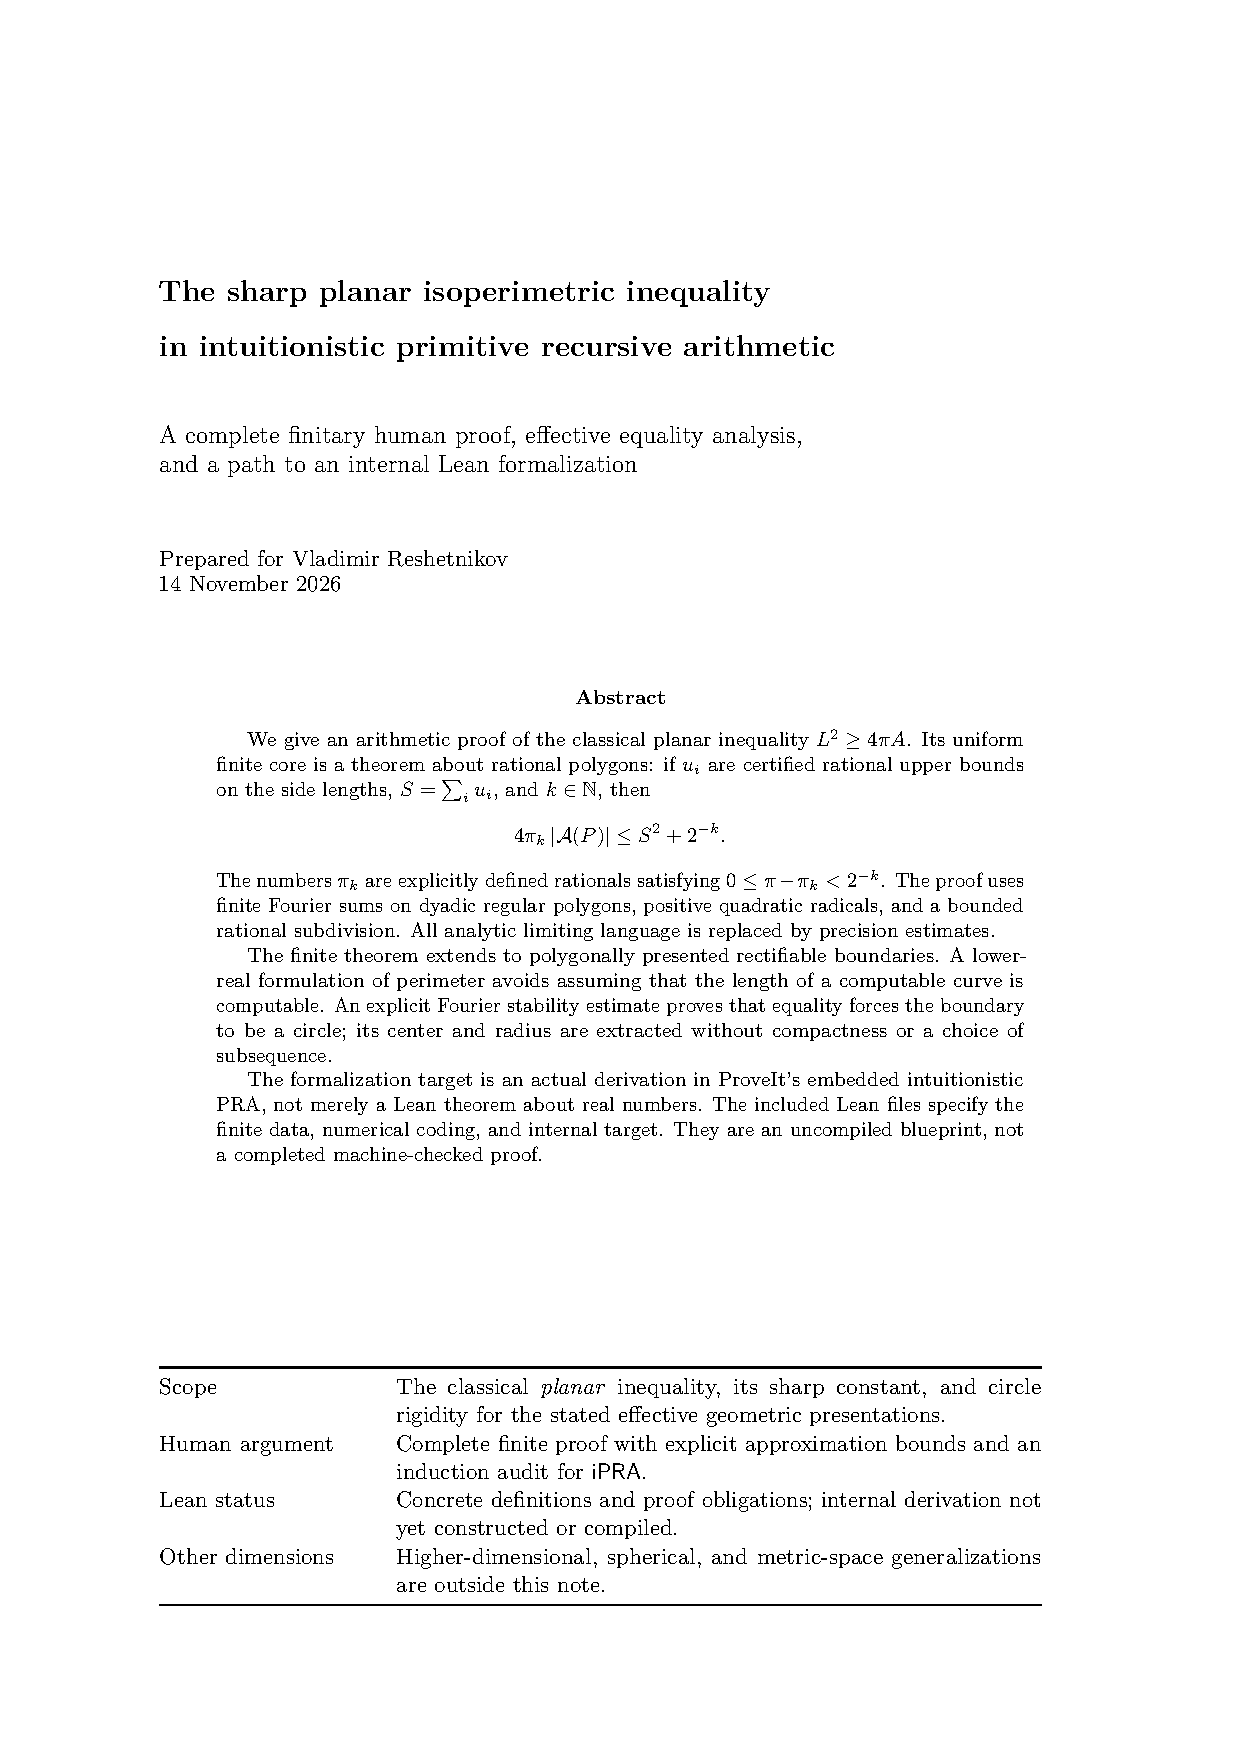
\includepdf[pages=-,pagecommand={\thispagestyle{empty}}]{../reused/isoperimetric_ipra.pdf}
\end{document}

